%!TEX root = ../main.tex

\chapter{Musical expectation}
\label{ch:5}

As opposed to the work presented in Chapter \ref{ch:3}, the study discussed in Chapter \ref{ch:4} led to the identification of differences between tracks previously reported as being able to cause MECs and tracks matched to those by artist, duration, and popularity, lending support to the intuition that such differences are more easily detected using computational methods on a large corpus of music. The work presented so far has considered each piece of music as a single data point, i.e., each piece of music was characterised by a one-dimensional vector of extracted features and behavioural responses. But, as discussed in Chapter \ref{ch:2}, MECs correspond to transient events occurring dynamically at particular points within a piece of music.

This chapter presents a computational analysis aimed at modelling the onset of MECs based on acoustic and musical characteristics (see Chapter \ref{ch:2}). We used the dataset of pieces of music initiated in Chapter \ref{ch:3}, labelled with onsets of MECs, and extracted features corresponding to previously identified acoustic and musical elicitors of MECs, as well as features capturing widely hypothesised elicitors of MECs, such as musical expectation. In the first part of the present study, we ran a series of permutation tests for each feature around the onsets of MECs, confirming in a systematic way, and at a much larger scale, the correlational effects that have been identified in previous research. In the second part, we compared the performance of two classification approaches, by training two different types of models on excerpts centred around the onsets of MECs and randomly selected excerpts from the same pieces of music, and testing these models in an automatic MEC onset detection task, resulting in the findings that the onsets of MECs could be predicted better than chance, and that musical expectation was the most effective predictor of MECs. 

\section{Introduction}
\label{se:exp-intro}

A major motivation for the present study was to compare the predictive performance of the previously identified elicitors of MECs. In order to do so, it is worth expanding on Chapter \ref{ch:2} by briefly reviewing these elicitors with a view to selecting a list of appropriate features for the analyses presented in this chapter.

\subsubsection{Acoustic elicitors}

Acoustic elicitors of MECs refer to low-level properties of the auditory signal. In early research on MECs, Sloboda (\citeyear{sloboda1991}) identified a relationship with sudden dynamic changes, by analysing music scores for passages reported to elicit MECs by survey participants. This relationship was confirmed empirically in subsequent research \parencite{auricchio2017,bannister2018,beier2020,grewe2007,guhn2007,honda2020,nagel2008,polo2017}, in which loudness was extracted \parencite[or manually inspected from music scores in the case of][]{guhn2007} around the onset of MECs experienced by participants when listening to music in a lab environment, which they reported either retrospectively, or continuously by pressing a button or moving a slider.

Loudness is by far the most documented acoustic correlate of MECs, but other relationships were also identified using similar methods, suggesting that occurrences of MECs tend to correlate with increases in roughness, dissonance, or fluctuation strength \parencite{bannister2018,beier2020,grewe2007,nagel2008,park2019}, increases in sharpness or brightness \parencite{bannister2018,beier2020,grewe2007,honda2020}, high spectral centroid and spectral flux \parencite{bannister2018}, high event density \parencite{bannister2018,nagel2008,polo2017}, or expansion of the frequency range in a high or low register \parencite{guhn2007,polo2017}.

In a recent study, \textcite{bannister2020b} experimentally manipulated loudness and brightness in two musical passages that had elicited MECs in previous research \parencite{bannister2018}. It was found that in one of the musical passages, MECs were experienced more frequently if loudness was increased, or if brightness was decreased (in contradiction with previous findings), therefore demonstrating a causal effect of loudness and brightness on MECs, as opposed to the correlational findings discussed above.

\subsubsection{Musical elicitors}

Musical elicitors of MECs refer to high-level properties of the musical structure. Sloboda (\citeyear{sloboda1991}), in the same study discussed above, identified that musical passages causing MECs also included new or unprepared harmonies, sudden textural changes, melodic appoggiaturas, enharmonic changes, specific melodic or harmonic sequences, or prominent events arriving earlier than prepared for, in decreasing order of frequency.

These self-reported effects of melodic and harmonic properties on MECs were confirmed in subsequent survey-based and empirical research \parencite{auricchio2017,bannister2020a,bannister2018,guhn2007,mlejnek2013,schurtz2012}, notably through the identification of an effect of structural transitions and alterations such as changes in tonality \parencite{bannister2020a}. Rhythmic properties \parencite{schurtz2012,solberg2019} and vocals \parencite{bannister2020a,schurtz2012} were also found to be involved, although there is a lack of specificity regarding which exact properties were associated with MECs. 

Additional findings revealed effects of crescendi, build-ups, and climaxes \parencite{auricchio2017,bannister2020a,bannister2018,panksepp1995,polo2017,solberg2019}, as well as textural changes \parencite{auricchio2017,polo2017,sloboda1991,solberg2019}, notably through the entrance of new instruments or the interplay between solo and background instruments \parencite{auricchio2017,bannister2020a,bannister2018,goodchild2019,guhn2007,mlejnek2013}.

\subsubsection{Emotional elicitors}

It is also worth mentioning emotional elicitors of MECs, which refer to subjectively perceived valence, emotionality, and meaning in music (see Chapter \ref{ch:2}). These characteristics of musical stimuli are difficult to quantify precisely and objectively, especially as continuous features, since they rely on some degree of subjective interpretation. Acoustic and musical elicitors, however, refer to properties of the auditory signal and of the musical structure that do not exclusively rely on subjective judgements.

For this reason, emotional elicitors were not considered in the present study, but we acknowledge that they are considered potent elicitors of MECs, and deserve further attention in future research.

\subsubsection{Expectation and chills}

As discussed in Chapter \ref{ch:2}, findings about musical elicitors have often been placed in the context of a hypothesised effect of musical expectation on MECs \parencite{harrison2014,huron2006,huron2010,juslin2008,juslin2013,mcdermott2012,mencke2019,pearce2012,salimpoor2011,sloboda1991}, positing that most of the musical elicitors listed above could be related to violations of expectation, and in turn, to experiences of MECs.

An effect of musical expectation on emotional responses to music has long been hypothesised \parencite{hanslick1854,meyer1956}, and has since been confirmed in empirical studies \parencite{cheung2019,egermann2013,gold2019,huron2006,juslin2013,sauve2018,steinbeis2006}. The effect of expectation on MECs, however, remains untested.

\subsubsection{Automatic detection of chills}

While the findings presented above represent a wide range of elicitors which are associated with MECs, most of these findings are qualitative or correlational in nature. In addition, elicitors were often identified by subjective analysis of music scores, and based on a relatively small amount of data. Despite these limitations, the degree of consensus for their effects on MECs suggests that automatic detection of MECs based on these elicitors might be possible.

The predictive modelling of continuous responses such as MECs, in addition to having received little attention in prior research \parencite{eerola2018}, requires large amounts of data, given the complexity in how acoustic and musical characteristics vary over time and interact with each other. This is especially relevant when also trying to investigate the relative influence of each individual elicitor on the occurrence of MECs.

While the ChiM dataset used in Chapter \ref{ch:4} is suitably large for such a task, it lacks consistent information about the exact versions of the pieces of music which elicit MECs, as well as precise information about the timing of MEC onsets. Using the dataset introduced in Chapter \ref{ch:3} addresses both of these challenges.

\subsubsection{Objectives}

The present study aimed to extract and process features representing acoustic and musical elicitors of MECs from an empirical dataset of onsets of MECs, to conduct a robust analysis of the effects of these elicitors on the occurrence of MECs, expecting these effects to replicate previous findings, and to uncover new evidence about an effect of musical expectation on MECs.

In addition, this chapter reports the design of a computational system for the automatic detection of MECs, which we expected to perform better than chance when predicting onsets of MECs based on acoustic and musical features. This system allowed the investigation of feature importance when predicting MEC onsets, through which we expected to observe a large influence of musical expectation. The models were cross-validated as a part of the training process, therefore reducing uncertainty in the findings due to the exploratory nature of this part of the present study.

First, we describe the additional data obtained through the survey study described in Chapter \ref{ch:3}. Then, we outline a set of features that broadly covered the range of elicitors discussed above. Finally, we detail the construction of analyses and models with the aim to provide a large-scale replication of current findings about the elicitors of MECs, to rank their importance in the elicitation of MECs, and to test the hypothesised effect of musical expectation on MECs.

\section{Methods}
\label{se:exp-methods}

\subsection{Stimulus selection}

\subsubsection{Dataset}

In order to collect a sufficient amount of training samples, considering the large number of features planned for model training, we left the survey study described in Chapter \ref{ch:3} running on Qualtrics (Qualtrics, Provo, UT) between February 2018 and April 2020. We collected a large number of self-reports of onsets of MECs from 2069 participants (including the 221 participants from Chapter \ref{ch:3}) ranging in age from 18 to 77 years (\emph{M} = 23.6 years, \emph{SD} = 8.8 years), and originating from a wide range of geographical areas (62 \% North America, 25\% Europe, 8\% Asia, 3\% Oceania, 1\% Africa, 1\% South America).

The resulting data required extensive manual cleaning. First, we removed entries from participants who abandoned the survey study before providing any piece of music, resulting in 1398 pieces of music being retained. Second, we removed entries which were not changed from the default answers provided in the questionnaire. Third, we processed the onsets of MECs, notably by converting time ranges to individual onsets, by removing some extraneous qualitative comments about specific musical characteristics leading to MECs, and by discarding a few entries which were higher than total track duration. Finally, we cleaned the URLs by removing further qualitative comments and by discarding non-valid URLs. This process resulted in retaining 1187 out of the 1398 reports of pieces of music causing MECs, corresponding to 1150 unique pieces of music associated with 2028 onsets of MECs.

Out of these, 1019 unique pieces of music could be retrieved for the present study, corresponding to 1806 onsets of MECs. We have made the data for these pieces of music available in \emph{Onsets of Chills in Music (oChiM)}, a dataset hosted permanently on the Open Science Framework.\footnote{oChiM is available at \url{https://doi.org/10.17605/osf.io/x59fm}}

\subsubsection{Stimulus preparation}

In order to be suitable for auditory feature extraction, tracks were retrieved as WAV files, downmixed to mono, and downsampled to 44.1 kHz when necessary, using the \emph{tuneR} R package \parencite{ligges2018}. RMS normalisation was then applied to all tracks simultaneously, using the \emph{soundgen} R package \parencite{anikin2019}. This process consisted of rescaling all audio files so that they had the same peak amplitude, set at 0 dB, and rescaling them linearly once more so that the RMS amplitude of each file matched that of the file with the lowest RMS amplitude.

\subsection{Feature extraction}

Based on the acoustic and musical elicitors of MECs reviewed above, we extracted a range of features which we believed most closely captured notions of loudness, roughness, brightness, spectral centroid and flux, event density, frequency range, crescendi, tonality, harmony, texture, expectation, and the presence of vocals.

\subsubsection{MiningSuite}

Most features were extracted using \emph{MiningSuite} \parencite{lartillot2019}, a MATLAB framework for the analysis of audio and music recordings, which expands on the methods provided by the commonly used \emph{MIRtoolbox} \parencite{lartillot2008}. Default settings for frame size were used for these features, as detailed below.

Loudness and crescendi were approximated with the \emph{aud.envelope} function, which consists of a generic envelope extraction method, further processed following a model of human auditory perception \parencite{klapuri2006}. The feature was extracted with a frame size of 10 ms, corresponding to a sampling rate of 100 Hz.

Spectral frame decomposition was then applied using the \emph{sig.spectrum} function, which applies a Fast Fourier Transform to the audio waveforms of each file, using a sliding window size of 50 ms with 25 ms overlap. This spectral decomposition was used to approximate the following elicitors: roughness with the \emph{aud.roughness} and \emph{sig.flatness} features, respectively estimating sensory dissonance and spectral smoothness; brightness with the \emph{aud.brightness} and \emph{sig.centroid} features, the former capturing the amount of high-frequency energy in the signal and the latter more broadly capturing spectral centroid (another elicitor of interest); spectral flux with the \emph{sig.flux} feature, calculating the spectral distance between successive frames; event density with the \emph{sig.entropy} feature, computing the relative Shannon entropy of the input \parencite{shannon1948}; and frequency range with the \emph{sig.spread} feature, capturing variance in the spectrum. These features were all extracted using the same sliding window size of 50 ms with 25 ms overlap as the initial spectral decomposition.

Tonality was approximated with the \emph{mus.key} feature, which estimates tonal centre positions by choosing the highest key candidate from a key strength curve, itself computed by correlating the chromagram of the signal with known key profiles \parencite{gomez2006,krumhansl1990}. This feature used a sliding window size of 1 s with 0.5 s overlap. Finally, to approximate harmonic change, a six-dimensional tonal centroid was first extracted using the \emph{mus.tonalcentroid} function, corresponding to chord projections on the circle of fifths, minor thirds, and major thirds, before being processed with the \emph{mus.hcdf} harmonic change detection function (HCDF), which returns the flux of the tonal centroid, using the default settings of a 743 ms sliding window size with 74.3 ms overlap.

Due to the computationally intensive nature of extracting many features from many tracks, the scripts were run in parallel on a series of Linux-based compute servers provided by Queen Mary University of London.

\subsubsection{Spleeter}

To generate a continuous, binary feature representing the presence of vocals, tracks were first processed using the \emph{Spleeter} source separation library \parencite{hennequin2020}, written in Python. The library provides pre-trained models to perform source separation of a music track into two, four, or five stems containing separate instruments. For the present study, two-stem separation was conducted, resulting in two separate tracks containing vocals and accompaniment for each track.

We applied an amplitude threshold to the tracks containing vocals only, in order to generate a binary feature reflecting the absence or presence of vocals which would discard the small amount of residual noise left in the tracks. In practice, since amplitude is characterised by a high degree of zero-crossing, which is not suitable for thresholding, we first computed the loudness of the vocals from their amplitude using the \emph{soundgen} R package, which provides a function allowing the estimation of subjective loudness in sones (a psychoacoustic unit of perceived loudness) for each 20 ms sliding window with 50\% overlap, resulting in a value capturing subjective loudness every 10 ms. To prevent the application of a loudness threshold from returning an overly sensitive vocals detection feature, we then applied a rolling maximum filter with a span of 510 ms for each track, before finally applying a loudness threshold, categorising vocals as present if above 2.5 sones, and absent if not. This thresholding process is visualised in \autoref{fig:exp-1}, and resulted in a continuous, binary feature representing the presence of vocals with a frame size of 10 ms.

\begin{figure}[t!]
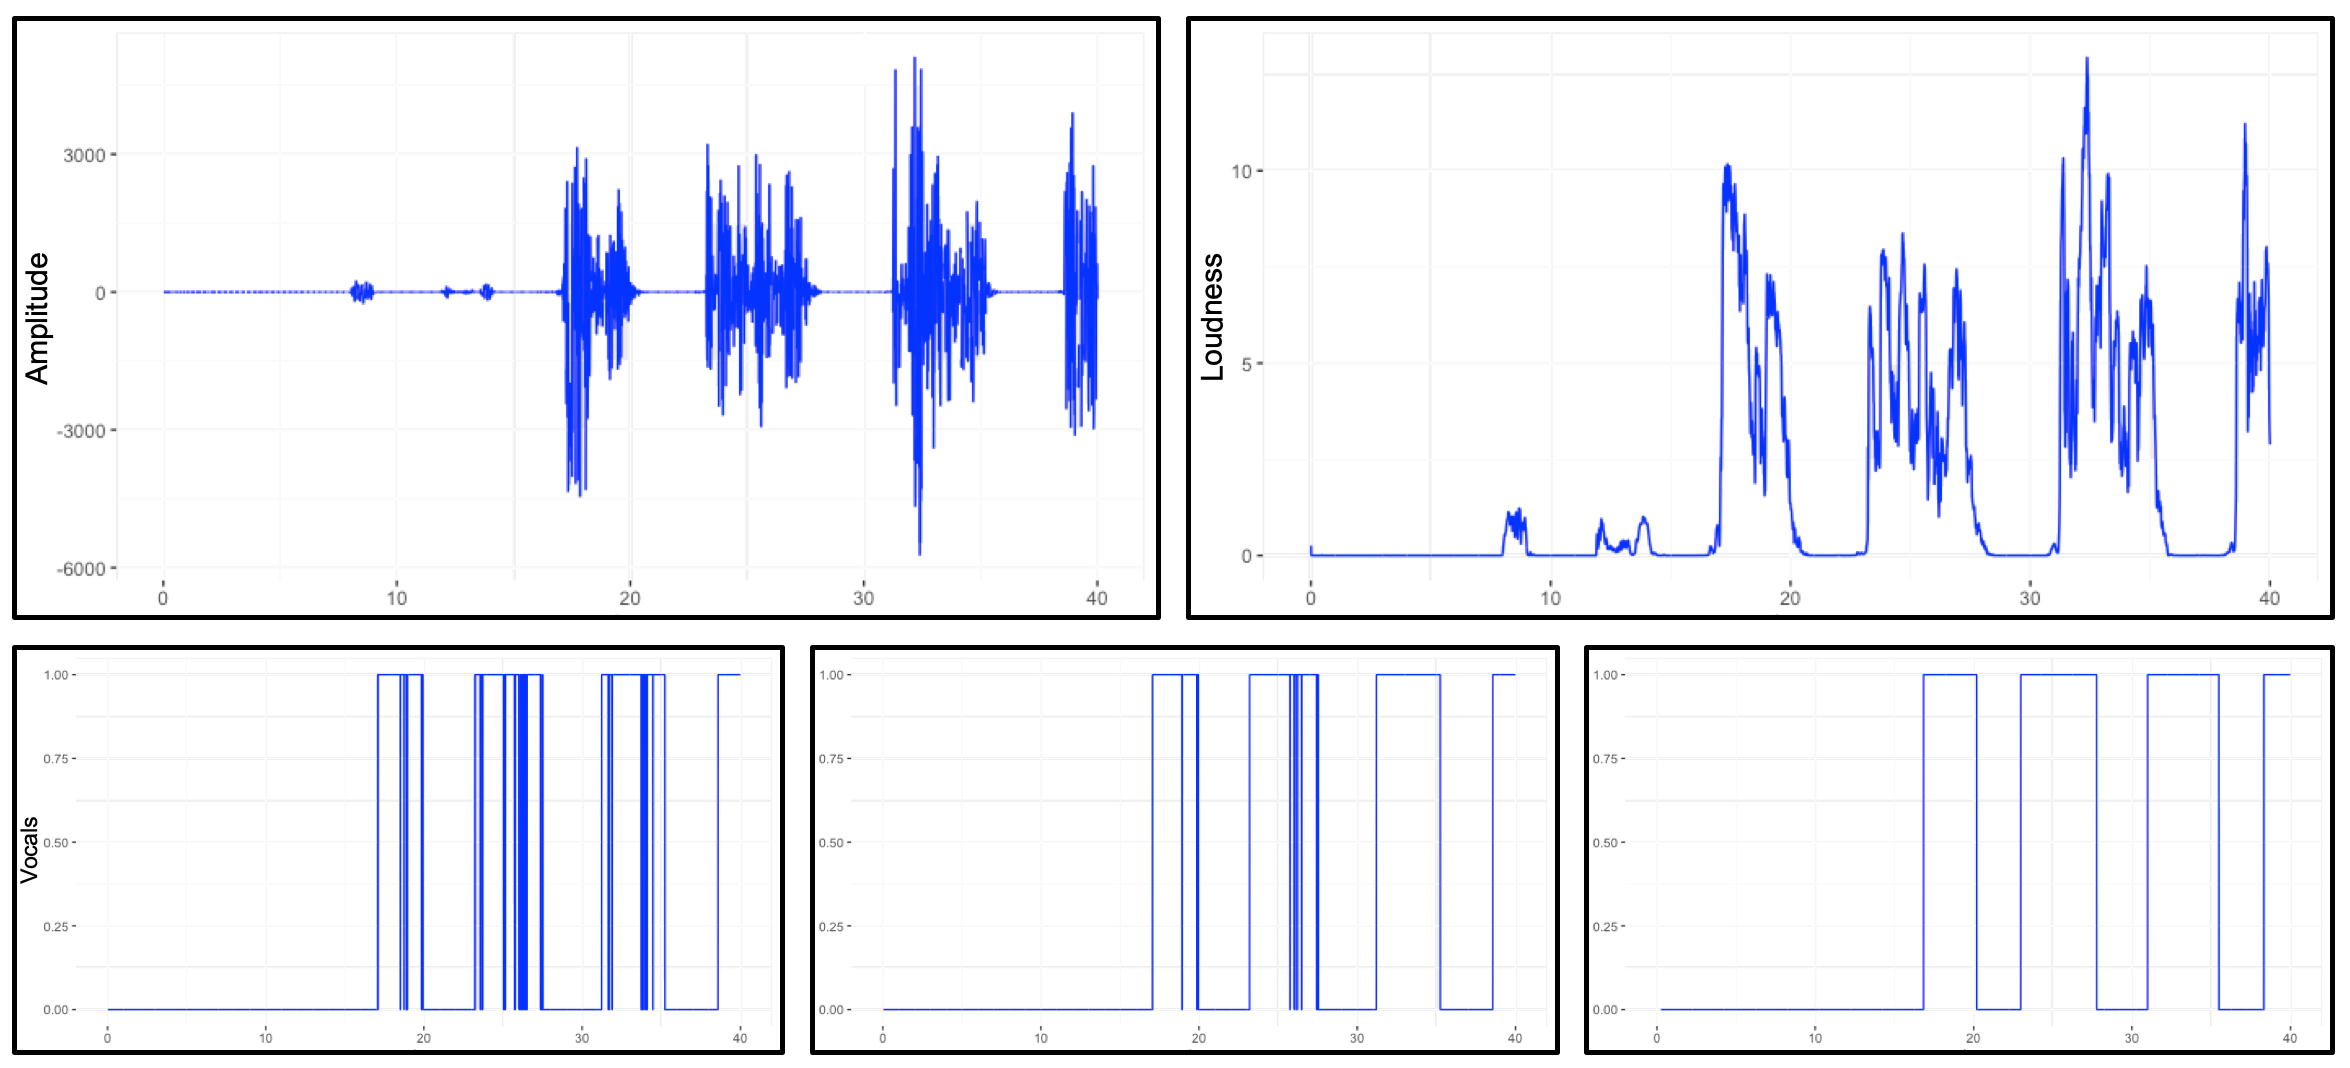
\includegraphics[width=\textwidth]{exp-1.png}
\centering
\caption{Vocals thresholding process. Data is shown for a short, 40-second excerpt in order to illustrate the thresholding process used to identify the presence of vocals. The top row shows the amplitude of the wave form of the vocals track extracted using Spleeter on the left, and an estimate of subjective loudness on the right. The bottom row shows the results of applying a loudness threshold at 2.5 sones with no rolling maximum filter on the left, a rolling maximum filter with a 50 ms span in the middle, and the same filter with a 510 ms span on the right. Several combinations of values were tested before the values used in the last plot were retained, as they were deemed to most closely approximate what manual annotation would return.}
\label{fig:exp-1}
\end{figure}

Note that both the 510 ms value for the span of the maximum filter and the 2.5 sones value for the loudness threshold were chosen manually, after comparing the outputs when changing these two parameters. A systematic validation was not possible due to the absence of labelled data in our sample. However, we conducted several manual checks on a representative set of recordings, and deemed the feature resulting from these parameters as close as possible to what would have resulted from manual annotation of the tracks. This allowed us not to allocate a disproportionate amount of time to the extraction of a single feature in the wider context of the present analysis. Note also that, while this feature is sensitive to differences in loudness between tracks, such concerns were mitigated by the fact that RMS normalisation was conducted prior to this step of the analysis.

\subsubsection{IDyOM}

Finally, in order to extract information about melodic expectation, it was necessary to extract melodies in MIDI format from each audio track. First, the time-series of continuous frequency values in Hz was extracted for each melody using the \emph{MELODIA} plugin \parencite{salamon2012} for \emph{Vamp},\footnote{\url{https://vamp-plugins.org}} via its associated \emph{vamp} Python library.\footnote{\url{https://pypi.org/project/vamp}} MELODIA enables the estimation of the fundamental frequency of the pitch of the primary melody in polyphonic tracks, and was therefore particularly well-suited for this task.

Then, a simple heuristic provided by the author of MELODIA\footnote{\url{https://github.com/justinsalamon/audio_to_midi_melodia}} was re-implemented in R in order to quantise pitch frequencies into discrete MIDI notes. This heuristic consisted of converting each value in Hz to its closest MIDI note before applying a median filter with a 250 ms span in order to remove some of the noise in the underlying data, and finally discarding notes shorter than 100 ms in duration. The resulting MIDI notes were stored in a text file suitable for the next step of the feature extraction process, while note onsets were stored in a reference file separately to convert the extracted features back to time-series suitable for model training.

\emph{IDyOM}, standing for Information Dynamics of Music \parencite{pearce2005,pearce2018}, was used to extract information about melodic expectation from these sequences of MIDI events. IDyOM is a system based on variable-order Markov models, which learns from the statistical regularities in symbolic, sequential events such as MIDI representations of melodies, and applies that knowledge to estimate the likelihood of each event within a sequence. This takes the form of two distinct measures, among other outputs of the model: \emph{entropy}, a measure of uncertainty about which event is predicted to come next given the current context at a specific position in a sequence, and \emph{information content}, a measure of the amount of information that is provided by an event given its previous context, which can therefore be used to quantify the surprisal of the event. For instance, if at time $t - 1$ in a melody, the system is very certain about which note comes next, this will be reflected by low entropy for that note occurring at time $t$. If the actual note in the sequence was indeed very predictable, this will be reflected by low information content, but if it was unexpected instead, information content will be high.

IDyOM provides a multiple-viewpoint system, which allows sequences to be modelled based on a range of melodic and rhythmic properties, such as pitch, chromatic pitch interval, contour, onset, duration, inter-onset interval, and many more. Options are provided for model training, including training a separate model on each sequence to make predictions for that sequence only (short-term model, capturing dynamic expectation), pre-training a model on a given corpus of sequences (long-term model, capturing schematic expectation), or combining both of these approaches. IDyOM has been the subject of substantial empirical testing, and was found to accurately predict melodic expectation in a range of experiments \parencite[for an extensive review, see][]{pearce2018}.

In the present study, the \emph{cpint} viewpoint (chromatic pitch interval) was derived from the \emph{cpitch} viewpoint (MIDI pitch number), in order to capture the entropy and information content of each MIDI event based on chromatic pitch interval. The model used a combination of the short-term and long-term models, with the long-term model being trained on a set of folk ballads from Nova Scotia, Bach choral melodies, and German folk songs from the Essen Folk Song Collection \parencite[for a description of this corpus, see][]{pearce2005}. The resulting entropy and information content values associated with each MIDI event for each tracks were linked back to the note onsets previously kept aside in a reference file, allowing these values to be converted to continuous features synchronised with the tracks.

The whole feature extraction process is visualised in \autoref{fig:exp-2}, along with the source of the features and the elicitors they were intended to approximate.

\begin{figure}[t!]
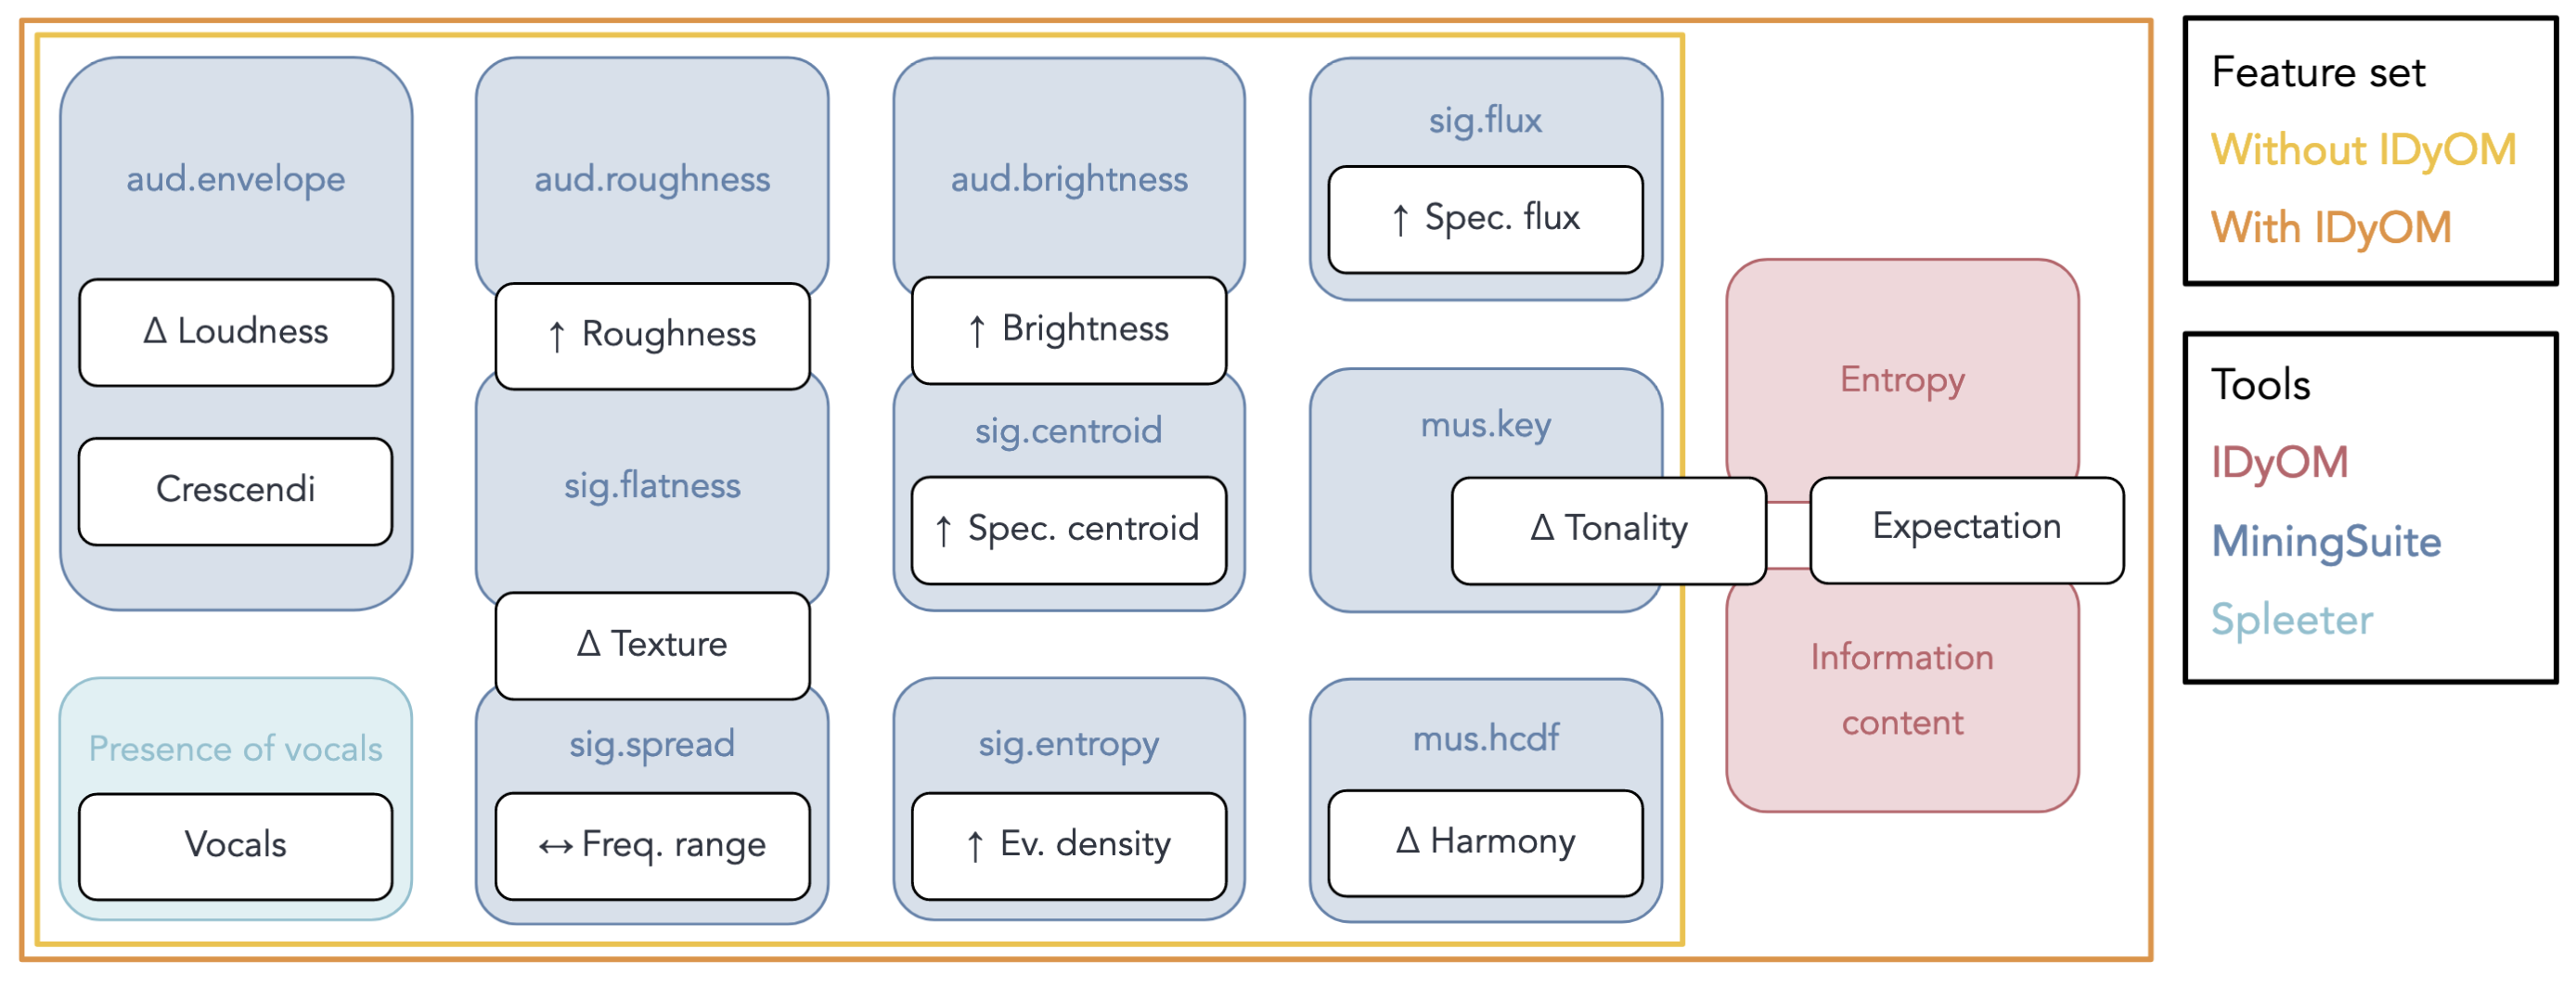
\includegraphics[width=\textwidth]{exp-2.png}
\centering
\caption{List of features extracted from each track. The features are shown in rectangular boxes with coloured backgrounds, corresponding to which tool was used to extract them. The acoustic and musical elicitors of MECs they aim to characterise are shown in white rectangular boxes (using the abbreviations \emph{freq.} for ``frequency'', \emph{spec.} for ``spectral'', and \emph{ev.} for ``event''), along with the hypothesised direction of their respective effects, as identified from prior research and shown with the following symbols: $\Delta$ for changes, $\uparrow$ for increases or elevated levels, and $\leftrightarrow$ for expansions. The outer rectangles represent the two feature sets used for model training, as described later in the present chapter.}
\label{fig:exp-2}
\end{figure}

\subsection{Feature preparation}

\subsubsection{Key distance}

Most features required additional processing in order to capture the hypothesised elicitors laid out in prior research. Tonality, notably, is only thought to affect the occurrence of MECs in occasional cases of changes in tonality. However, the current feature extracted with \emph{mus.key} only captured the tonal centre at a given time, which should have no bearing on the occurrence of MECs. We decided to compute key distance from this feature, following the intuition that more unexpected changes in tonality might be more conducive to experiencing MECs. To do so, we first smoothed the feature by applying majority voting with a 3.5 s span, before assigning a value to tonality changes based on distance on the circle of fifths. For instance, if the tonal centre at time $t - 1$ was C, the key distance at time $t$ would be 0 if the tonal centre remained C, 2 if it changed to D, or a maximum of 6 if it changed to F\#. The feature was then upsampled to 100 Hz for consistency with the other features, replacing the newly introduced missing values by their nearest existing key distance value.

\subsubsection{Interpolation and smoothing}

Cubic spline interpolation was applied to all the other auditory features extracted with MiningSuite in order to match this 100 Hz frame rate, with the exception of envelope, which was already sampled at 100 Hz. Care was taken only to allow the addition of new values in the gaps between two existing values, in order to prevent cubic spline interpolation from returning wildly unlikely values at the very beginning and end of each track, where more missing values might be found. Following this, all features (including envelope) were smoothed by using a median filter with a span of 50 ms.

\subsubsection{First-order difference}

As discussed earlier (and seen in \autoref{fig:exp-2}), many elicitors of MECs refer to changes in acoustic and musical properties, as opposed to specific values. To allow the analyses in the present study to detect this behaviour, first-order differences were computed for each feature and also included in the analyses, such that if a feature had a value of 3 at time $t - 1$ and a value of 7 at time $t$, its first-order difference at time $t$ would be $7 - 3 = 4$.

\subsubsection{Segmentation}

In order to speed up computations for the planned analyses, and to investigate both central tendencies and variance for each feature, summary statistics were computed over successive segments for each feature. All analyses in the present study were run twice: once with a segment size of 200 ms, and once with a segment size of 500 ms, since there was no information to determine a priori which segment size would work best to investigate the occurrence of MECs. For each segment, the mean and standard deviations were computed, resulting in four dimensions for each original feature: $\mu_0$ and $\sigma_0$, the mean and standard deviation of the original values, and $\mu_1$ and $\sigma_1$, the mean and standard deviation of the first-order difference. Note that due to the way key distance was generated, standard deviations were not computed as they would not contain any meaningful information. In the present study, $\mu_0$ can be thought of as the original feature, $\sigma_0$ as the variance in that feature, $\mu_1$ as the rate of change in the feature, and $\sigma_1$ as the variance in that rate of change.

In addition, we predicted that for three features (envelope, HCDF, and key distance), changes on a slower time scale might better capture their hypothesised role as elicitors of MECs. These features were therefore also segmented using a 2 s sliding window with 50\% overlap, and upsampled to both 200 ms and 500 ms frame sizes, in order to be included in both sets of analyses. The full list of features is shown in \autoref{tab:exp-1}. These features were used for both sets of analyses---one with features using a 200 ms frame size, and one with features using a 500 ms frame size, as a result of the two different types of segmentation. The table includes display names for each feature, which are used for plotting the results in the rest of the present chapter due to space constraints within the plots. The computed features have also been made available on oChiM.\footnote{\url{https://doi.org/10.17605/osf.io/x59fm}}

\begin{table}[h]
\centering
\small

\begin{threeparttable}
\caption{Display names for features included in both sets of analyses}
\label{tab:exp-1}

\begin{tabular*}{\textwidth}{@{\extracolsep{\fill}}llllll@{}}
\toprule
\textbf{Tool} & \textbf{Feature category} & \multicolumn{4}{l}{\textbf{Features}}\\ 
\cmidrule{3-6}

& & \textbf{$\mu_0$} & \textbf{$\sigma_0$} & \textbf{$\mu_1$} & \textbf{$\sigma_1$} \\ 
\midrule

MiningSuite & Envelope       & $\mu_0$env    & $\sigma_0$env    & $\mu_1$env    & $\sigma_1$env    \\
            & Envelope +     & $\mu_0$env+   & $\sigma_0$env+   & $\mu_1$env+   & $\sigma_1$env+   \\
            & Roughness      & $\mu_0$rough  & $\sigma_0$rough  & $\mu_1$rough  & $\sigma_1$rough  \\
            & Flatness       & $\mu_0$flat   & $\sigma_0$flat   & $\mu_1$flat   & $\sigma_1$flat   \\
            & Brightness     & $\mu_0$bright & $\sigma_0$bright & $\mu_1$bright & $\sigma_1$bright \\
            & Spec. centroid & $\mu_0$spcent & $\sigma_0$cent   & $\mu_1$cent   & $\sigma_1$cent   \\
            & Spec. flux     & $\mu_0$spflux & $\sigma_0$flux   & $\mu_1$flux   & $\sigma_1$flux   \\
            & Spec. entropy  & $\mu_0$spent  & $\sigma_0$spent  & $\mu_1$spent  & $\sigma_1$spent  \\
            & Spec. spread   & $\mu_0$spspr  & $\sigma_0$spspr  & $\mu_1$spspr  & $\sigma_1$spspr  \\
            & Key distance   & $\mu_0$kdist  &                  & $\mu_1$kdist  &                  \\
            & Key distance + & $\mu_0$kdist+ & $\sigma_0$kdist+ & $\mu_1$kdist+ & $\sigma_1$kdist+ \\
            & HCDF           & $\mu_0$hcdf   & $\sigma_0$hcdf   & $\mu_1$hcdf   & $\sigma_1$hcdf   \\
            & HCDF +         & $\mu_0$hcdf+  & $\sigma_0$hcdf+  & $\mu_1$hcdf+  & $\sigma_1$hcdf+  \\
Spleeter    & Vocals         & $\mu_0$voc    & $\sigma_0$voc    & $\mu_1$voc    & $\sigma_1$voc    \\
IDyOM       & Mel. entropy   & $\mu_0$melent & $\sigma_0$melent & $\mu_1$melent & $\sigma_1$melent \\
            & Mel. IC        & $\mu_0$melic  & $\sigma_0$melic  & $\mu_1$melic  & $\sigma_1$melic  \\
\bottomrule

\end{tabular*}
\begin{tablenotes}
\small
\item Note. Four types of features for each feature category. $\mu_0$ = mean of the original values, $\sigma_0$ = standard deviation of the original values, $\mu_1$ = mean of the first-order difference, $\sigma_1$ = standard deviation of the first order difference, + = feature segmented using a longer, sliding window, Spec. = Spectral, Mel. = Melodic, IC = information content.
\end{tablenotes}
\end{threeparttable}
\end{table}

\section{Analysis}

\subsection{Permutation tests}

In order to identify patterns in the behaviour of each feature around the onset of MECs, we ran a series of permutation tests \parencite[for a similar approach, see][]{grewe2009b}. As previously discussed in Chapter \ref{ch:3}, permutation tests consist of identifying a test statistic that captures the dimension we want to measure, and generating a null distribution by permuting samples, in order to assess whether or not the observed results were unlikely enough to reject the null hypothesis. Here, we explored each feature by evaluating how unlikely their values were around the onset of MECs, when compared to other moments within the tracks which were not reported as causing MECs.

To do so, we extracted all 20-second excerpts centred around the onsets of MECs from each track. We only retained complete excerpts, meaning that onsets of MECs within the first or last 10 seconds of each track were discarded. Rather than choosing individual control excerpts for each excerpt causing MECs, we split every track into sequential 20-second excerpts, discarded every excerpt which was not complete, or partially or fully overlapped with any of the excerpts causing MECs, and retained all the remaining excerpts as controls. This process therefore resulted in two unbalanced sets of 20-second excerpts, capturing 10 seconds before and after each onset of MECs for one set, and almost all other moments within the tracks for the control set.

The test statistic was computed for each frame of each feature, and consisted of the difference between the average values for excerpts causing MECs and control excerpts. Two-tailed permutation tests were run by randomly permuting the excerpts while keeping the same number of excerpts in each set, using Monte Carlo estimation with 5000 replications. We only ran the permutation tests on the data with a 500 ms frame size in order to limit the number of comparisons we would draw, and we used Bonferroni correction within each feature, to further mitigate the fact that, even with a 500 ms frame size, 41 significance tests would be required for each feature.

\subsection{Principal components analysis}

We trained models to assess whether or not the onsets of MECs could be predicted using audio-derived acoustic and musical features, and if so, which features were most important in driving such predictions. In addition to the two types of segmentations discussed above, we evaluated two types of models (described later in this section), on two sets of features. The first set of features did not include the IDyOM features, while the second set did. This was done in order to specifically evaluate the effect of accounting for expectation on the predictive performance of the models.  For clarity, we hereafter refer to these differences in model training as differences in \emph{frame size} (200 ms or 500 ms), \emph{feature set} (without or with IDyOM features), and \emph{model type} (described below).

We expected a high degree of collinearity in the features, with features in some cases being exactly identical, with the exception of the type of segmentation they were subjected to. As discussed in Chapter \ref{ch:4}, PCA is a convenient way to address collinearity, by retaining principal components above a set eigenvalue threshold. We therefore conducted four PCAs with centring and scaling---one for each combination of frame size (200 ms or 500 ms) and feature set (with or without IDyOM).

The results of the PCAs are discussed here for simplicity, as they are not crucial to the rest of the findings discussed in the present chapter. We retained 12 principal components with eigenvalues above one for each PCA using the first feature set (without IDyOM) regardless of frame size, and 15 principal components for each PCA using the second feature set (with IDyOM) regardless of frame size as well. Taken together, these principal components accounted for at least 75\% of cumulative proportion of variance explained for each PCA (see \autoref{fig:exp-3} for an example).

\begin{figure}[t!]
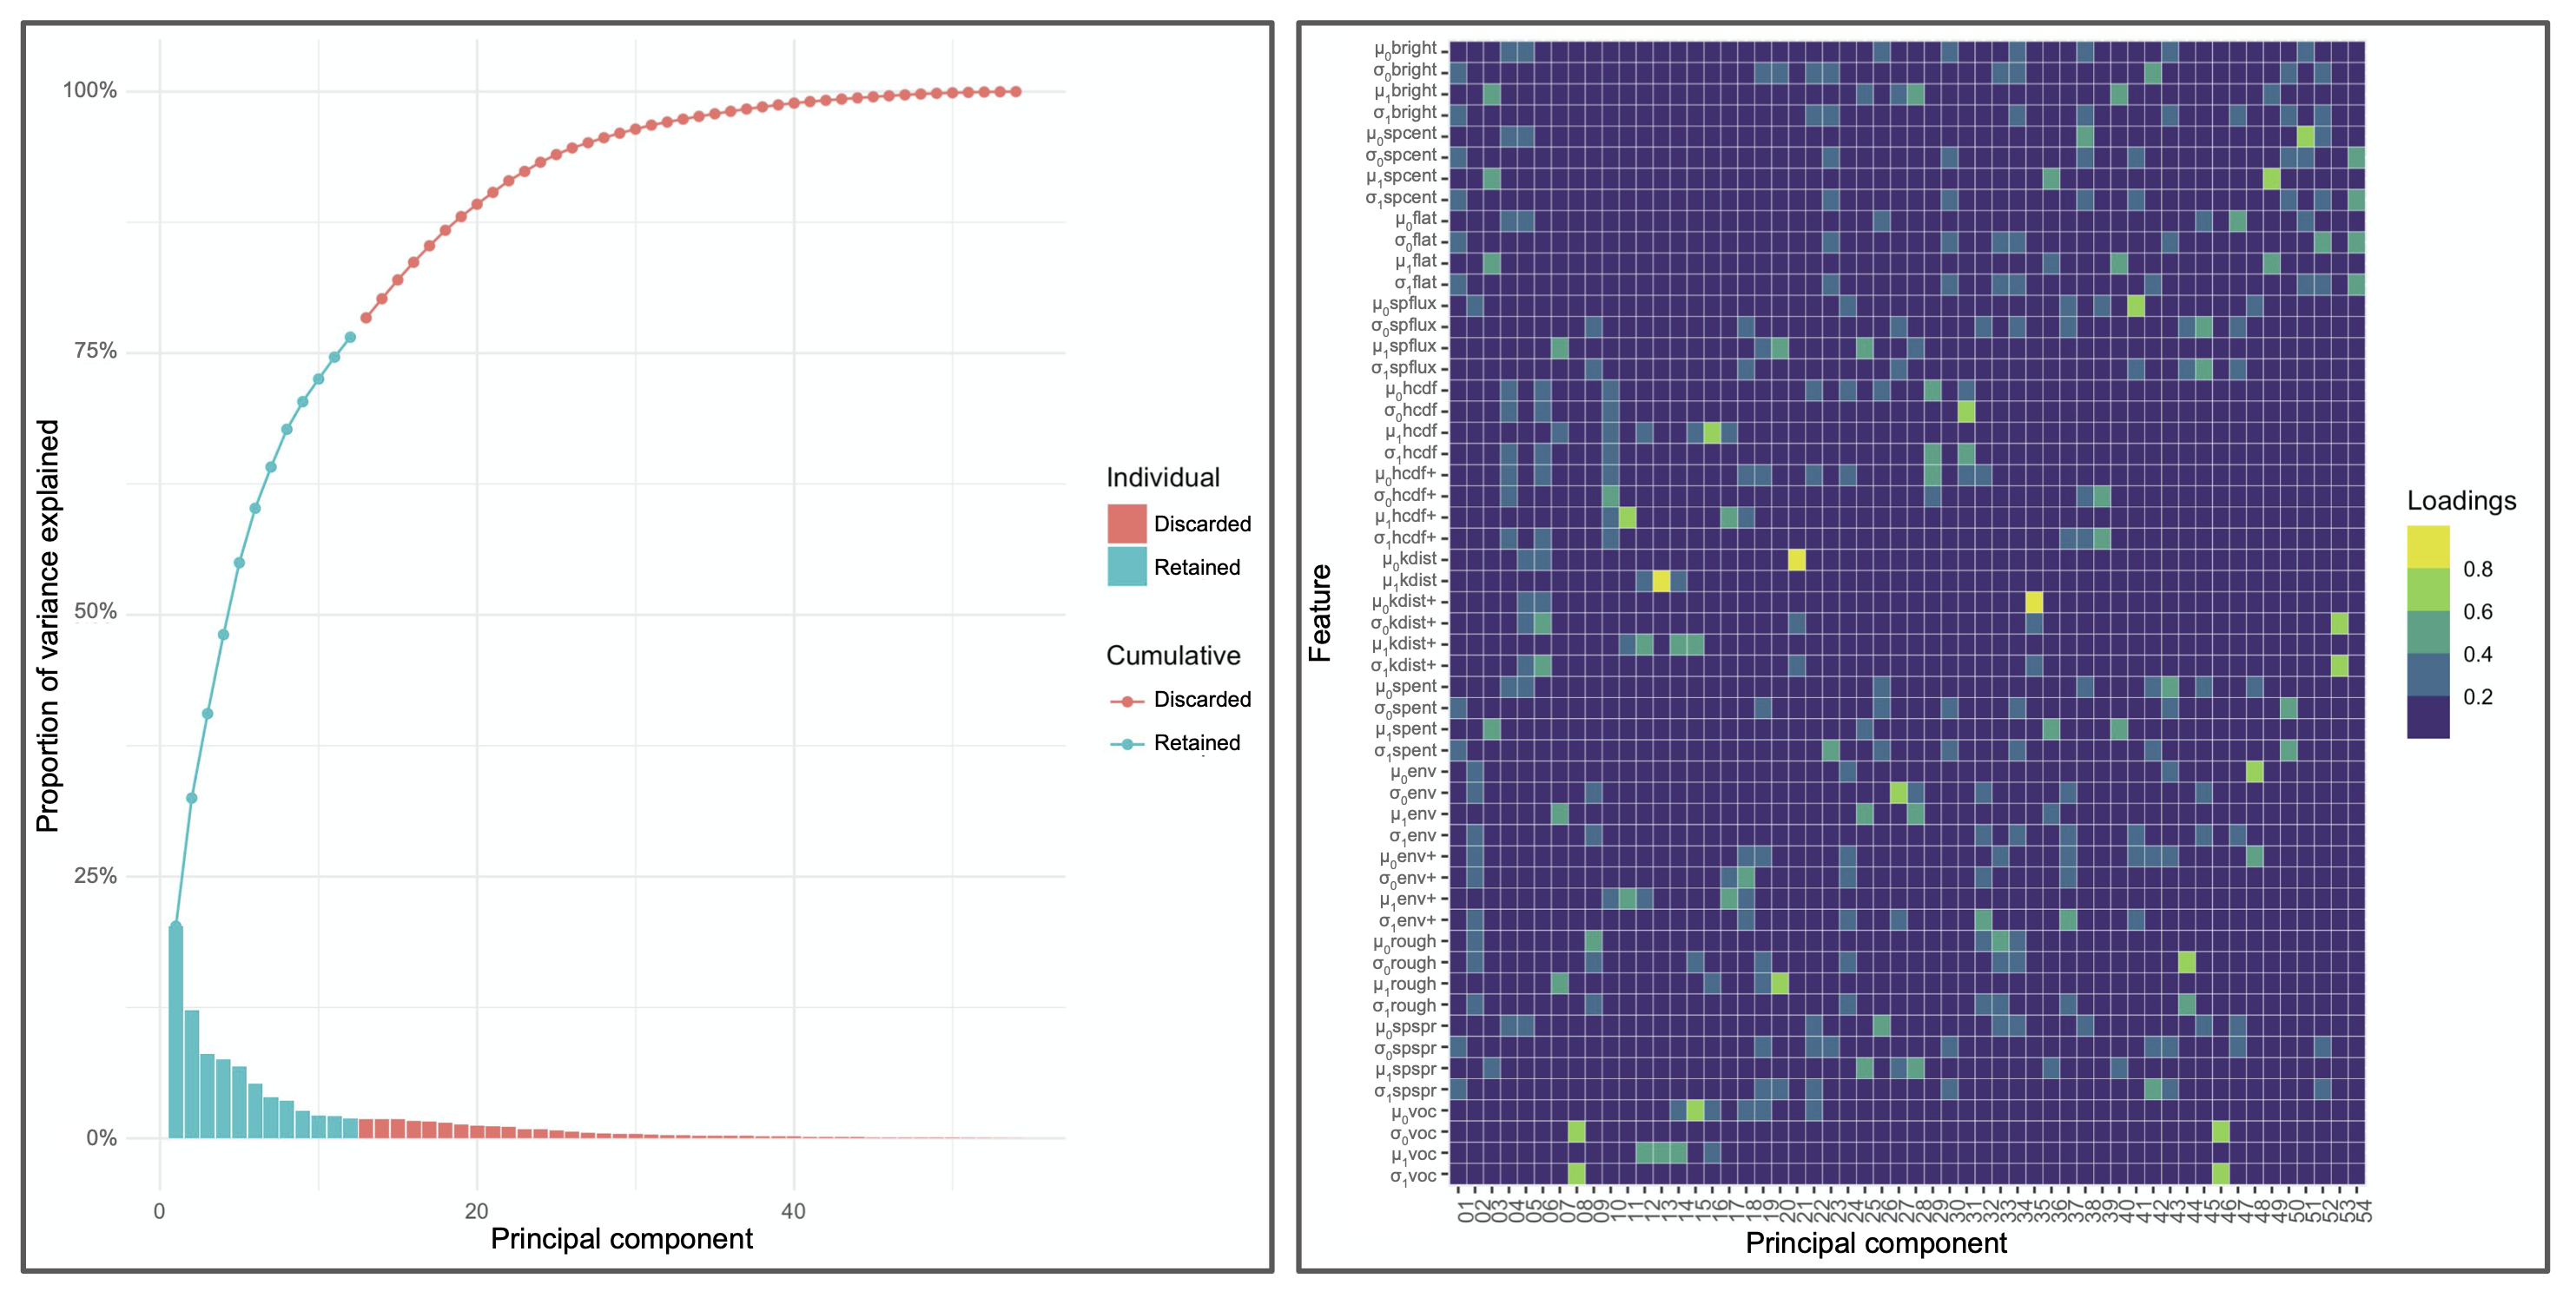
\includegraphics[width=\textwidth]{exp-3.png}
\centering
\caption{Visualisation of principal component analysis for one of the four combinations of feature set (without IDyOM features) and frame size (200 ms). On the left, a scree plot shows the 12 retained principal components, along with the proportion of variance explained they account for, both individually and cumulatively. On the right, a heat map displays feature loadings on each principal component.}
\label{fig:exp-3}
\end{figure}

While we didn't attempt to interpret how the features were grouped together into specific principal components, we stored feature loadings on each principal component and proportion of variance explained by each principal component for later analyses of feature importance.

\subsection{Hidden Markov models}

The first models we trained were hidden Markov models (HMMs). As opposed to Markov chains, which model the probabilities of sequences of observable states, HMMs model the probabilities of hidden states, which themselves drive the probability distributions of observable events. HMMs are specified by a set of of hidden states, the transition probabilities between these states, an initial probability distribution for these states, a set of observations, and the observation likelihoods associated with each state, also called emission probabilities–––the probability that an observation was generated by a specific state \parencite[for excellent introductions to HMMs, see][]{jurafsky2021,rabiner1989}.

In its most simple form, for a univariate sequence of observations, an HMM associates each hidden state with a specific emission distribution (e.g., normal distribution with a given mean and standard deviation) of the observed values in that sequence. In practice, we are often faced with multivariate sequences of observations, and instead of using multivariate Gaussian emissions, which might be limited in how accurately they can represent observations, Gaussian mixture model emissions (GMMs) are often used. GMM-HMMs are particularly well suited to modelling auditory events due to their flexibility and sequential nature, and have successfully been applied to speech recognition \parencite[see][]{juang1991}, or, in a music context, to segmentation, genre classification, sequence prediction, and event detection \parencite[e.g.,][]{ajmera2003,wang2019}.

It is worth clarifying what each component of an HMM represented in the present analysis. The observations corresponded to the multidimensional sequence of features (or rather, of principal components), different configurations of this multidimensional sequence were modelled by GMMs, each governed by a different hidden state of the HMM. It was assumed that specific sequences of hidden states gave rise to the occurrence of MECs (as opposed to having a single hidden state represent MECs specifically). 

Fundamentally, HMMs are characterised by three problems \parencite{jurafsky2021,rabiner1989}: the likelihood problem (determining the likelihood of a specific sequence of observations given the HMM and observations), the decoding problem (discovering the best hidden state sequence given the HMM and observations---not relevant to the present study because we did not attempt to interpret the hidden states themselves), and the learning problem (learning the HMM parameters given the states and observations). The present automatic MEC onset detection task consisted of two steps. In the first step, we trained two separate HMMs (learning problem). The first HMM was trained on excerpts centred around the onsets of MECs, and the second HMM on control excerpts. In the second step, we presented these trained HMMs with new excerpts to obtain the likelihood of each excerpt according to each HMM (likelihood problem). If the HMM trained on excerpts causing MECs returned the highest likelihood, the excerpt was categorised as inducing MECs, and vice versa. Implementation details are provided below.

As with the permutation tests, this approach required extracting two sets of excerpts, since HMMs are best trained on short sequences of equal length. The exact same procedure was used, selecting excerpts centred around the onset of MECs, and control excerpts sequentially through the rest of each track. However, instead of 20-second excerpts, we tested two excerpt durations: two seconds (with a frame size of 200 ms only), and five seconds (with a frame size of 200 ms or 500 ms), in order to speed up computations while ensuring a reasonable amount of frames would be retained for each excerpt. \emph{Excerpt size} (2 s or 5 s) therefore corresponds to the last aspect of model training we controlled, in addition to frame size, feature set, and model type.

In the survey from which onsets of MECs were gathered, participants reported these onsets with a time resolution of one second. We therefore decided to augment the training data by also extracting excerpts categorised as causing MECs for each frame within one second of the original onset of MECs. For instance, with a frame size of 500 ms, instead of getting a single excerpt for an onset of MECs at $t =$ 40 s, we extracted five excerpts at $t =$ 39, 39.5, 40, 40.5, and 41 s. This also allowed us to reduce the severe class imbalance, with control excerpts outnumbering excerpts causing MECs by a ratio of 100:1.

Using the \emph{pomegranate} Python library \parencite{schreiber2018}, a pair of HMMs (MECs and control) was trained for each combination of feature set (with or without IDyOM), frame size (200 ms or 500 ms), and excerpt size (2 s or 5 s), using manual grid search by iterating over the number of hidden states and the number of Gaussian mixtures the models should be trained with. More specifically, in order to save time on this very computationally intensive training process, we trained each model using odd numbers of states and mixtures (ranging from 1 to 17), before testing the even numbers of states and mixtures nearest to the best performing model. This process is illustrated in \autoref{fig:exp-4}. We used five-fold cross-validation, using for each fold 60\% of the tracks as a training set, 20\% as a validation set to pick the best performing model for testing, and 20\% as a testing set to return final performance metrics for the combination of learning parameters which performed best across all five folds. As with feature extraction, model training was run in parallel on university-provided compute servers.

\begin{figure}[t!]
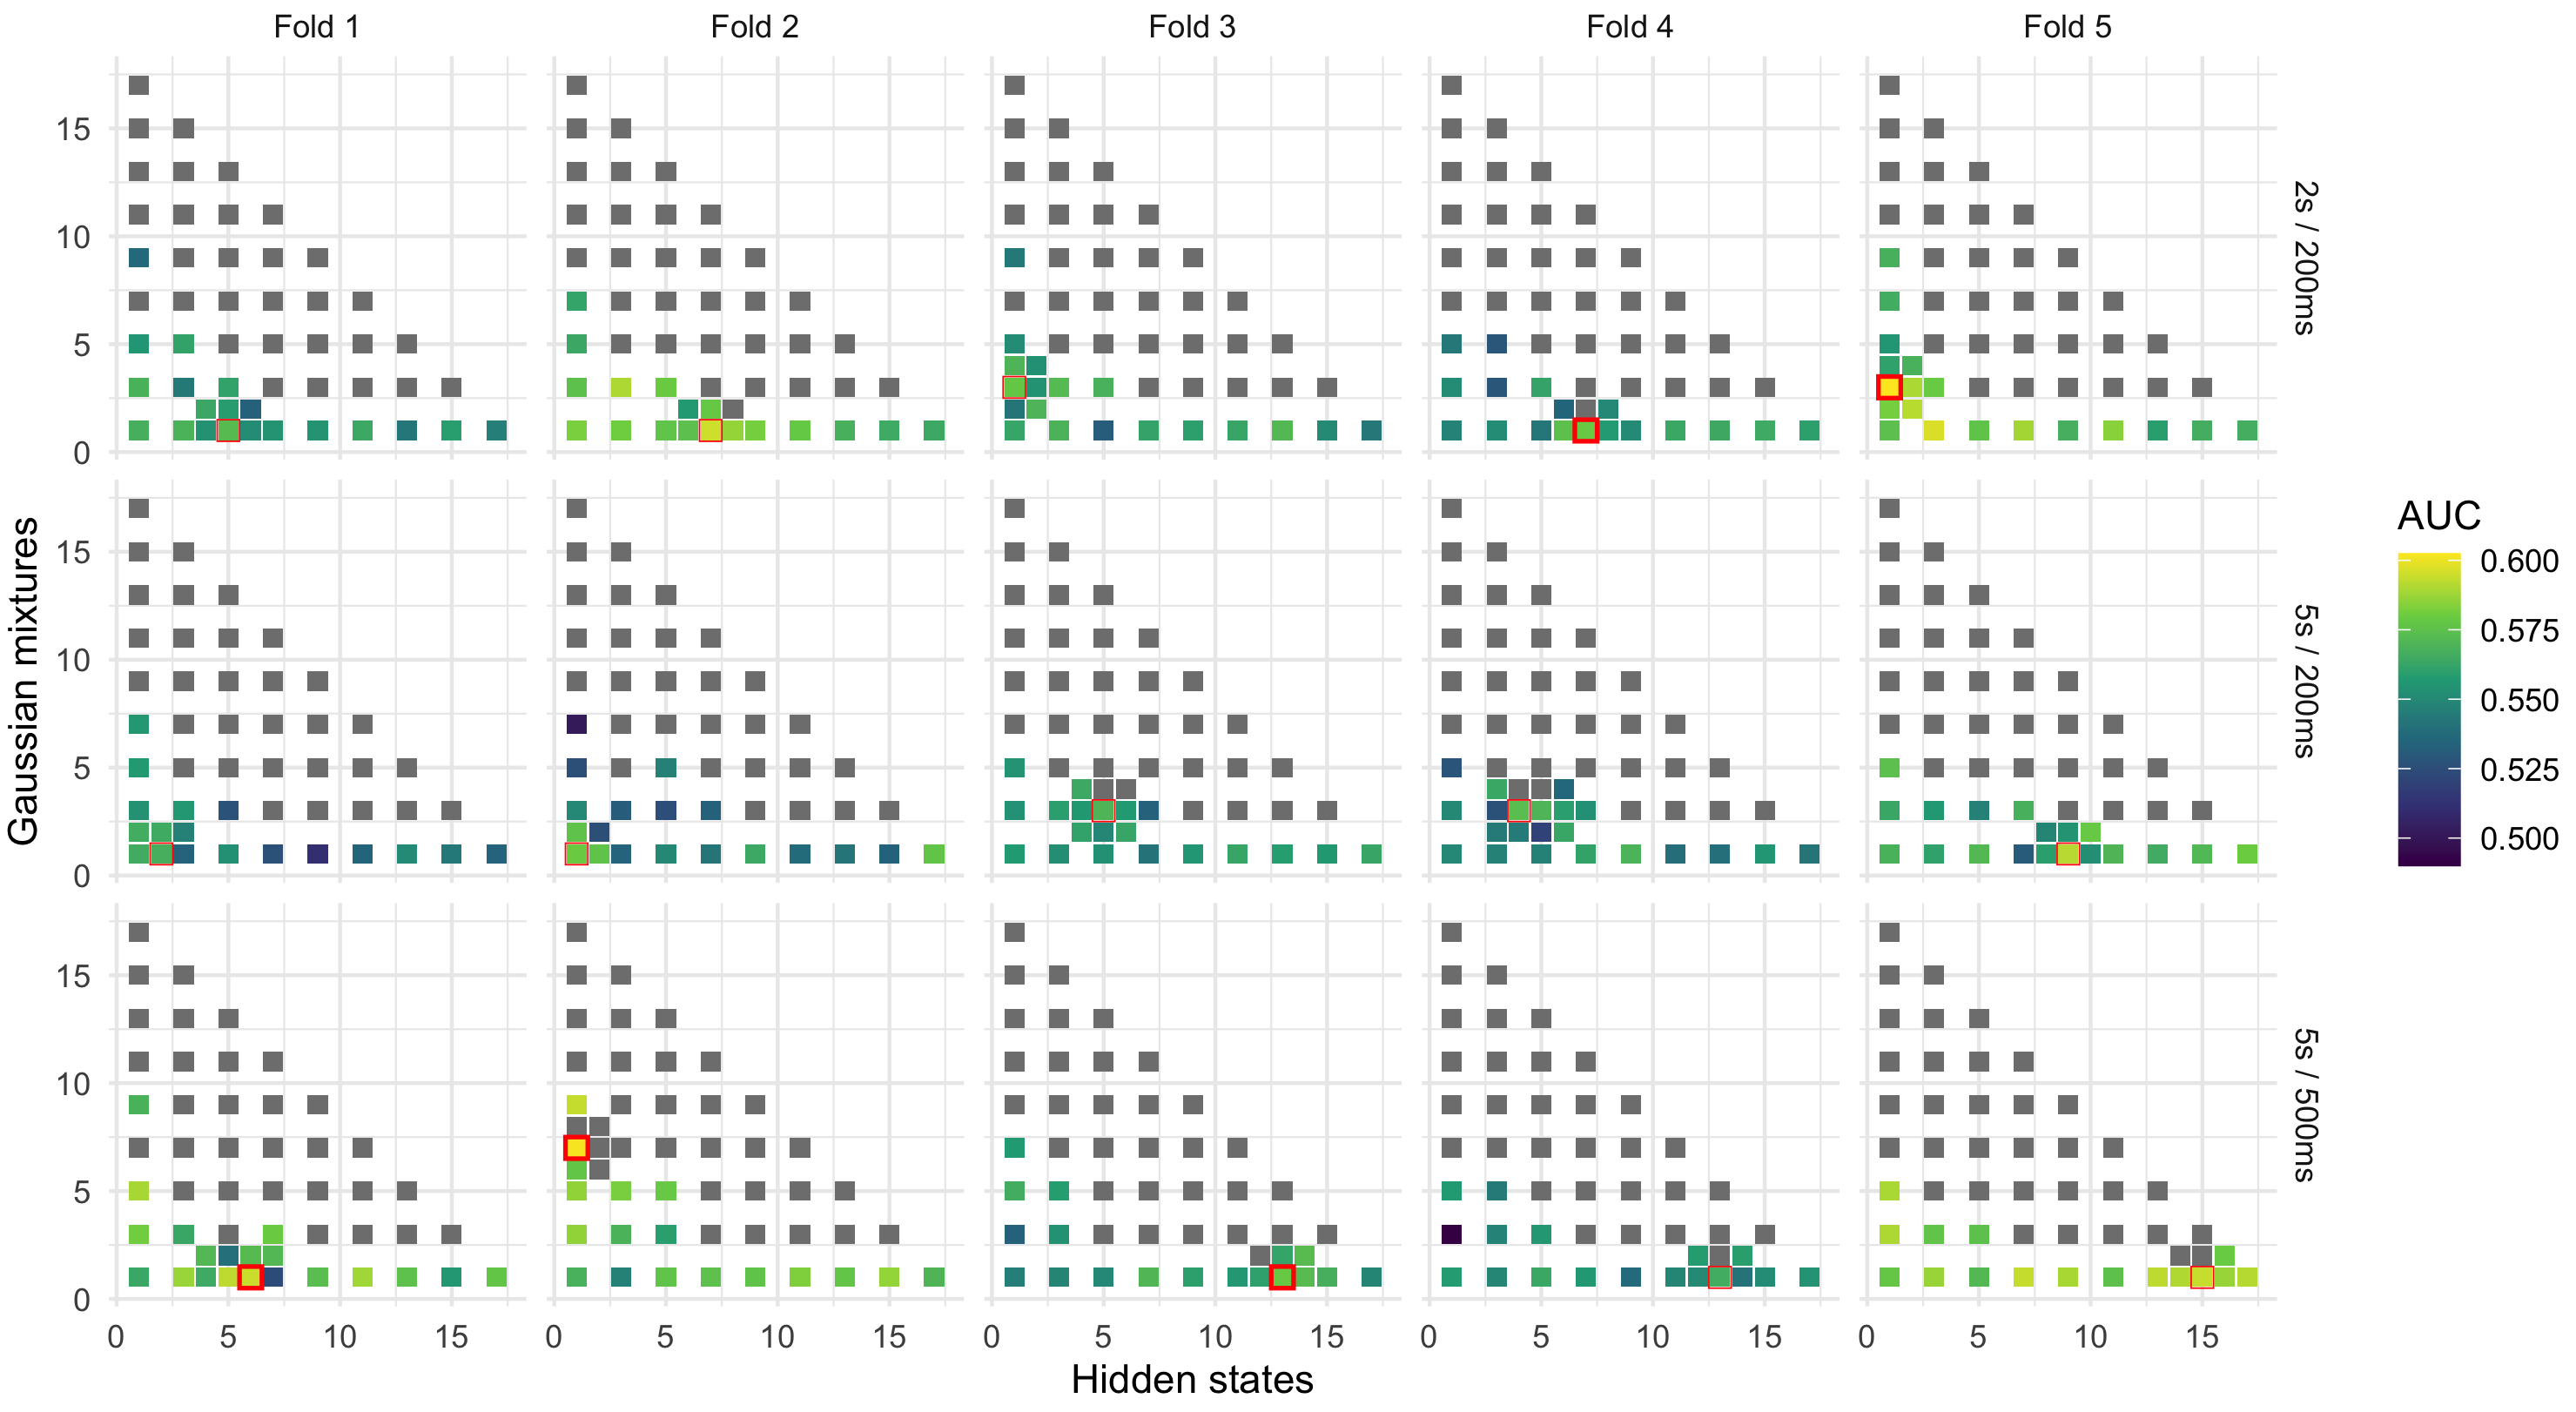
\includegraphics[width=\textwidth]{exp-4.png}
\centering
\caption{Grid search for GMM-HMM training. In this example, HMMs were trained on the feature set which includes IDyOM features. A pair of HMMs (MECs and control) was trained for each combination of number of hidden states (bottom axis), Gaussian mixtures (left axis), cross-validation fold (top axis), and excerpt size and frame size (right axis). Model performance was evaluated using area under the receiver operating characteristic curve (AUC). Odd numbers of states and mixtures were first used for training. For each combination of fold, excerpt size, and frame size, additional models were trained using the even numbers of states and mixtures closest to the best performing models (highlighted in red), resulting in some cases in increased performance (e.g., see Fold 1, 5 s excerpt size, 500 ms frame size). Cell colour represents models which failed to converge, in grey, or AUC. The best performing HMMs for each fold are highlighted with a thicker, red border.}
\label{fig:exp-4}
\end{figure}

The process for training an individual HMM was as follows. All data was concatenated, ignoring its sequential nature, to identify a cluster for each hidden state using k-means, and initialise the parameters of the corresponding GMM using said cluster. The model was then initialised with a uniform probability transition matrix, before training began using the Baum-Welch algorithm \parencite[see][]{jurafsky2021}. Regularisation was applied, by setting a transition and emission pseudocount of 0.1, and an edge and distribution inertia of 0.1 \parencite[see][]{schreiber2018}. If the model failed to converge, generally due to underflow errors, training was attempted once more. If unsuccessful, training was abandoned and a new model was trained for the next step of the grid search, as seen in \autoref{fig:exp-4}.

Full tracks, split into consecutive excerpts, were used for model validation. For each excerpt from each track in the validation test, a log probability value was obtained for each of the pair of trained HMMs (the one trained on excerpts causing MECs, and the one trained on control excerpts), using the forward algorithm \parencite[see][]{jurafsky2021}. If the HMM trained on excerpts causing MECs returned the highest log probability for the tested excerpt, that excerpt was predicted as an occurrence of MEC, and vice versa. For each fold, this validation process resulted in a univariate time-series of binary predictions for each track.

Due to the sequential nature of the resulting predictions, two sets of performance metrics were computed, using the \emph{sed\_eval} Python library \parencite{mesaros2016}: \emph{event}-based metrics, and \emph{segment}-based metrics. Event-based metrics compare ground truth and predictions frame by frame, usually allowing for a \emph{collar}---a small amount of tolerance around the onset of a predicted occurrence of MECs. We opted for a one-second collar, which resulted, for instance, in predicted occurrences of MECs being categorised as true positives if they were within one second of an onset of MECs in the ground truth. Segment-based metrics compare ground truth and predictions in a fixed time grid, marking segments are active if they include an onset of MECs, and inactive if not. We opted for a five-second segment length, resulting in a given segment being categorised as a true positive if it included an onset of MECs in both the ground truth and the predictions.

For both types of metrics, we computed precision, recall, and F-measure---the harmonic mean of precision and recall. In addition, for segment-based metrics, we computed balanced accuracy, which is not available for event-based metrics \parencite[see][]{mesaros2016}, as well as true positive rate and false positive rate, in order to compute the area under the receiver operating characteristic curve (AUC). In a typical classification task, the AUC is calculated by modifying the classification threshold. In the present analysis, however, predictions were not made based on a classification threshold, but rather by comparing log probabilities between two HMMs. To emulate the principle of a classification threshold, we collected all frame-wise log probability differences and extracted their percentiles. Each percentile was used as a proxy for a threshold, by generating a new set of predictions based on whether or not the difference between the log probabilities of both HMMs was higher or lower than that percentile. This allowed us to collect 100 pairs of true positive rates and false positive rates (one for each percentile), which were then used to compute the AUC with the \emph{scikit-learn} Python library \parencite{pedregosa2011}.

After observing the results, discussed later in the present chapter, we also decided to compute F\textsubscript{$\beta$}, which applies an additional weight $\beta$ to the F-measure in order to disproportionately favour precision or recall over the other. We picked a value of 2 for $\beta$---a standard value to signify that we considered recall twice as important as precision in the present analysis. This decision and its implications are explored in the discussion. For the validation sets, only AUC was used to select the combination of learning parameters which performed best across all five folds. For each fold, the HMMs trained using these learning parameters were then used on the testing set to compute the AUC. All other performance metrics were computed for the classification threshold (i.e., the log probability difference threshold) which returned the highest F\textsubscript{$\beta$} value. These metrics were then averaged across all five folds to return final model performance metrics.

\subsection{Support-vector machines}

For purposes of comparison, we ran all analyses using a second type of model called support-vector machine (SVM). For classification tasks using an SVM, model training consists of finding the hyperplane which maximises the distance between the two classes, and is used as a decision boundary to make predictions. SVMs are widely used for classification tasks, and were chosen in the present analysis as a more naive modelling approach because, when compared to HMMs, they are much quicker to train, less prone to fitting errors, relatively easy to interpret, and have the added benefit of being more forgiving in terms of statistical assumptions than logistic regression---another commonly used classification method. However, as opposed to HMMs, they do not take into account the sequential nature of the data.

SVMs were trained using \emph{scikit-learn} with a linear kernel, no random feature selection, a stopping criteria set at $10^{-5}$, and by adjusting weights inversely proportional to class frequencies in order to account for class imbalance. The HMM workflow detailed above was replicated to train, validate, and test SVMs, with a few exceptions. First, separating the training data into excerpts was not necessary, since SVMs could be trained on the whole dataset at once. This also meant that instead of generating several excerpts to account for the imprecision in the time resolution of onsets of MECs, we simply assigned positive labels to all frames within one second of the onset of MECs. Second, grid search was performed, but only involved varying feature set (with or without IDyOM), frame size (200 ms or 500 ms), and the regularisation parameter for linear SVMs (using a logarithmic scale ranging from $10^{-24}$ to $10^{4}$, with even-numbered exponents only). Third, predictions were made frame-wise, but we still used event-based and segment-based evaluation metrics. Finally, as discussed earlier, computing the AUC requires modifying the classification threshold, but linear SVMs do not return the probabilities associated with the predictions for each frame by default. To obtain these probabilities, we applied Platt scaling \parencite{platt1999} on the decision function, and then computed the AUC similarly as for the HMMs, by adjusting the classification threshold over the percentiles of these probabilities.

\subsection{Feature importance}

The final step of the analysis was to extract feature importance. To simplify the interpretation of the results, feature importance was only extracted from the best performing model across all combinations of excerpt size, frame size, feature set, and model type. Since the best performing model ended up being an SVM, as revealed in the results, the method described below is specific to feature importance extraction from the parameters of a trained SVM.

Using Platt scaling involves a second layer of cross-validation within each cross-validation fold. We refer to the folds from this second layer as \emph{SVM folds} to differentiate them from the cross-validation folds used in the workflow detailed above. First, feature coefficients were extracted from the parameters of the trained models. Since we were interested in assessing feature importance, as opposed to trying to interpret the directionality of the coefficients (which was more relevant to the permutation test analyses), absolute values were taken, therefore preventing coefficients from cancelling each other out when averaged over SVM folds, if directionally different. These absolute values for the coefficients of each feature were averaged over each SVM fold, resulting in a set of five positive, averaged coefficients for each feature, i.e., one coefficient per cross-validation fold.

However, in this case, the features were principal components obtained with PCA. To tie the coefficients back to the original features, we had to apply weights to these coefficients based on proportion of variance explained by and feature loadings on each principal component, thereby assigning a share of the influence of each principal component on the models to its constituent features, based on how much variance in the data that principal component accounted for. To do so, we simply took the feature loadings on each principal component, multiplied them by the proportion of the variance explained by each principal component, and multiplied that by the coefficients extracted from the models for that principal component. We then added up the coefficients for each feature across all principal components, resulting, again, in a single coefficient per feature for each of the cross-validation folds (but this time, for each of the original features, as opposed to principal components).

The magnitude of the coefficients differed between cross-validation folds, but since the folds were of equal size, and we were interested in feature importance, we rescaled the coefficients linearly for each fold, such that 0 corresponded to the least contributing feature for that fold, and 1 to the most contributing feature. Finally, we averaged these values across the five cross-validation folds, resulting in a single feature importance value, between 0 and 1, for each of the original features that were used for PCA before model training. Note that these values do not exactly correspond to a rank, but rather, to a continuous spectrum of feature importance, where a value of 0 would represent the feature with the lowest feature importance on all five cross-validation folds, and a value of 1 for the highest feature importance.

\section{Results}

Far too many permutation tests were conducted to meaningfully present the results in a table. Instead, we opted to visualise all the results in \autoref{fig:exp-5}. This figure warrants extensive explanation, and is therefore discussed here rather than in the figure caption. Note that all feature values were Z-scored in the figure, in order to better visualise the magnitude of the effects, and to enable better comparisons across features.

\begin{figure}[t!]
\includegraphics[width=\textwidth]{exp-5.jpg}
\centering
\caption{Visualisation of the permutation tests. Vertical blue lines denote frames for which there were significant differences between the excerpts causing MECs (thick blue line) and control excerpts (thin grey line).}
\label{fig:exp-5}
\end{figure}

Each plot within the grid corresponds to one of the features that was included in the PCA (keeping in mind that we only ran permutation tests on the dataset with a 500 ms frame size). The plots are arranged by rows, corresponding to feature categories, and by columns, corresponding to summary statistics. The x-axes represent 20-second excerpts, centred around the onsets of MECs, and the y-axes represent Z-scores. Within each plot, the horizontal line at $y = 0$ therefore represents a Z-score of 0, and the vertical dotted line at $x = 0$ represents the onsets of MECs.

The thin grey time-series represent values averaged over all the control excerpts, while the thicker blue time-series represent values averaged over all the excerpts centred around reported onsets on MECs. For a given frame, a significant difference in average feature values between these two time-series, as revealed by a permutation test, is indicated by a vertical blue line. As mentioned earlier, permutation tests were not conducted for $\sigma_0$\emph{kdist} and $\sigma_1$\emph{kdist} due to the way these features were computed.

Interpretation of these results is provided in the discussion, but we can already easily identify several features showing higher values in the excerpts causing MECs, or sharp increases around the onset of MECs.

The results for the predictive modelling of the onsets of MECs are presented in \autoref{tab:exp-2}, which shows evaluation metrics for the best performing combinations of model type (HMM or SVM), feature set (with or without IDyOM features), and metrics type (segment-based or frame-based). Including IDyOM features in the feature set resulted in slightly better metrics overall, with the exception of AUC for the HMM, which was slightly lower with IDyOM features. Both SVMs outperformed the HMMs, with the SVM trained using all features reaching a segment-based AUC of 0.597, F\textsubscript{$\beta$} of 0.167, and balanced accuracy (the arithmetic mean of the accuracy on each class) of 0.580. All models exhibited very low precision and good recall, therefore leading to low F-measures and motivating the choice of F\textsubscript{$\beta$} as an evaluation metric, as expanded upon in the discussion. Interestingly, the best performing models for each category, as described in \autoref{tab:exp-2}, all used the features with a 500 ms frame size, as opposed to 200 ms.

\begin{table}[h]
\centering
\footnotesize

\begin{threeparttable}
\caption{Evaluation metrics and learning parameters for each model}
\label{tab:exp-2}

\begin{tabular*}{\textwidth}{@{\extracolsep{\fill}}lllrrrrrr@{}}
\toprule
\textbf{Model} & \textbf{IDyOM} & \textbf{Metric type} 
  & \multicolumn{6}{l}{\textbf{Evaluation metrics}}\\ 
\cmidrule{4-9}

    &           &         & AUC            & $F_{\beta}$    & $F$            & $P$            & $R$            & $BA$           \\ 
\midrule

HMM & \ding{55} & Segment & 0.579          & 0.161          & 0.075          & 0.040          & 0.682          & 0.564          \\
    &           & Frame   & -              & 0.091          & 0.042          & 0.022          & 0.442          & -              \\
    & \ding{51} & Segment & 0.577          & 0.165          & 0.076          & 0.040          & \textbf{0.744} & 0.571          \\
    &           & Frame   & -              & 0.099          & 0.046          & 0.024          & 0.429          & -              \\
SVM & \ding{55} & Segment & 0.592          & 0.166          & 0.078          & 0.041          & 0.713          & 0.579          \\
    &           & Frame   & -              & 0.080          & 0.036          & 0.019          & 0.466          & -              \\
    & \ding{51} & Segment & \textbf{0.597} & \textbf{0.167} & \textbf{0.078} & \textbf{0.041} & 0.693          & \textbf{0.580} \\
    &           & Frame   & -              & 0.088          & 0.041          & 0.022          & 0.383          & -              \\
\bottomrule

\end{tabular*}
\begin{tablenotes}
\small
\item Note. Highest values in bold. HMM = Hidden Markov model, SVM = Support-vector machine, AUC = Area under the receiver operating characteristic curve, $F_{\beta}$ = F\textsubscript{$\beta$}-measure, $F$ = F-measure, $P$ = Precision, $R$ = Recall, $BA$ = Balanced accuracy.
\end{tablenotes}
\end{threeparttable}
\end{table}

In order to maximise the amount of data that could be used for model training, we opted for the cross-validation approach described above, testing the trained model on a different section of the dataset for each cross-validation fold, instead of training a final model to obtain evaluation metrics on a holdout set. Therefore, as explained earlier, AUC was computed from five different receiver operating curves instead of a single one. These curves are shown in \autoref{fig:exp-6}, along with the threshold which resulted in the highest F\textsubscript{$\beta$} values for each curve.

\begin{figure}[t!]
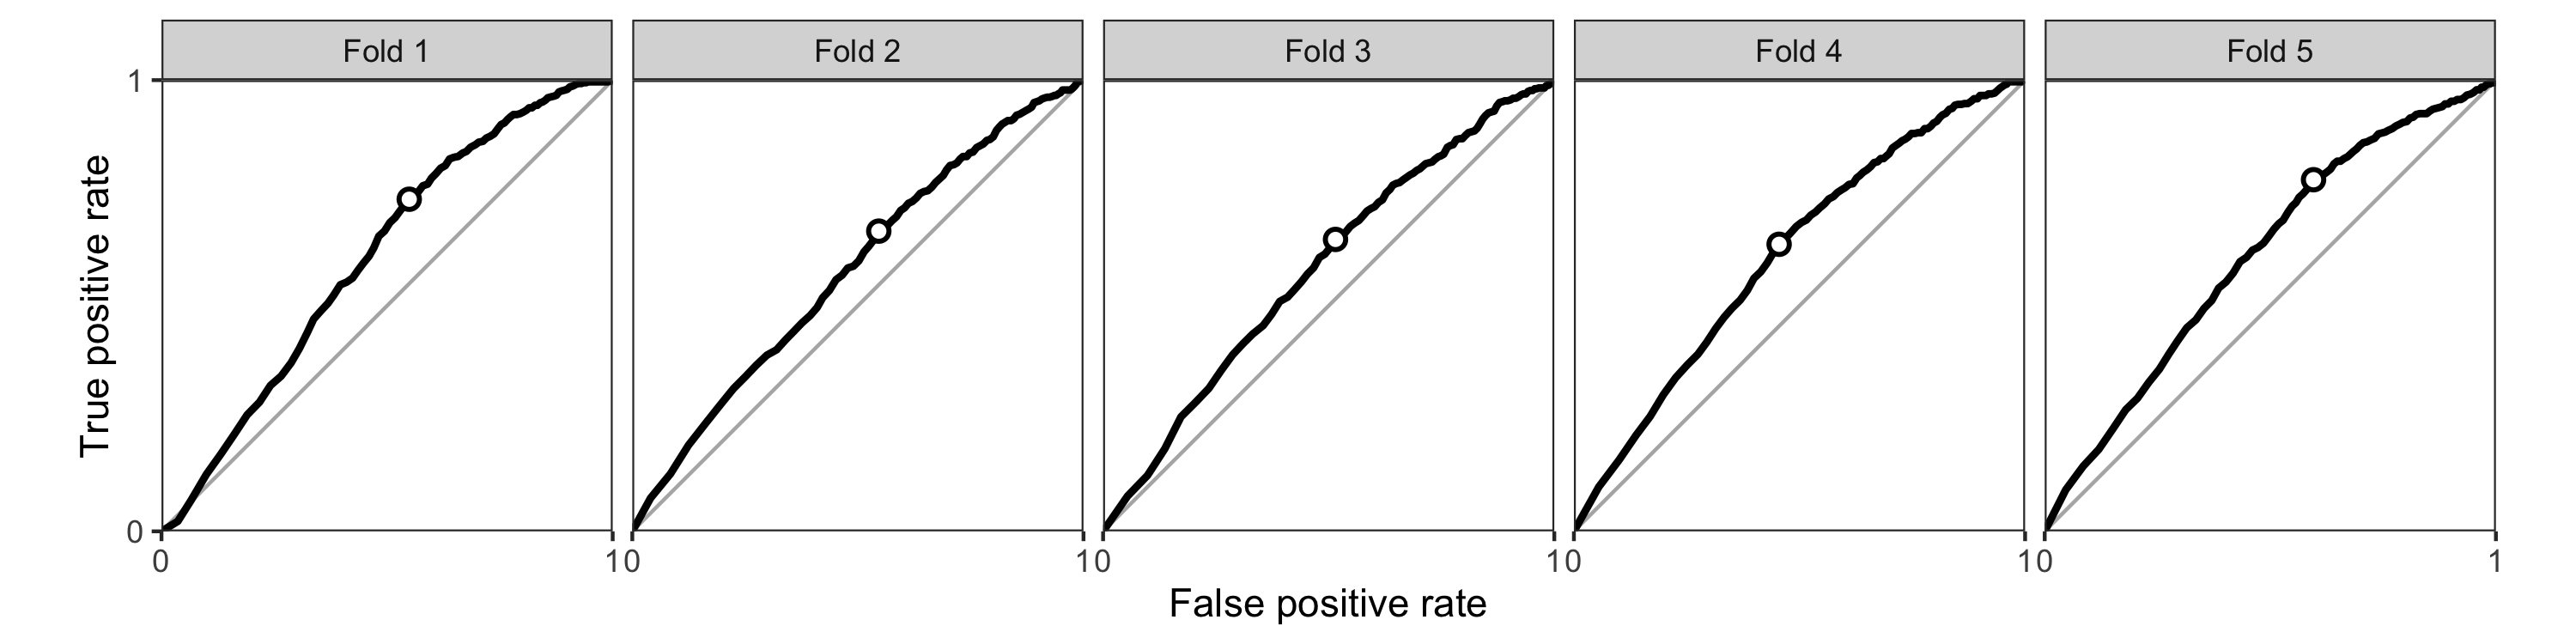
\includegraphics[width=\textwidth]{exp-6.png}
\centering
\caption{Receiver operating curves for each cross-validation fold of the SVM trained using all available features. Overall AUC for the model was computed by averaging the AUCs for each curve. The threshold which returned the highest F\textsubscript{$\beta$} value is visualised by a circle on each curve, and corresponds to the threshold at which all evaluation metrics were retained before being averaged to return overall evaluation metrics for the model.}
\label{fig:exp-6}
\end{figure}

Finally, the contribution of each feature to the best-performing SVM is visualised in \autoref{fig:exp-7}, in terms of feature importance. Melodic entropy and information content, as computed with IDyOM, were the best predictors of MECs, with melodic entropy reaching a value of 1, meaning it was the most important predictor on all five cross-validation folds. Following these two features were the variance of the first-order difference of melodic entropy, as well as mean spectral flatness, spread, and centroid. The least contributing features were the mean first-order differences of brightness, roughness, and spectral entropy, spread, and centroid.

\begin{figure}[t!]
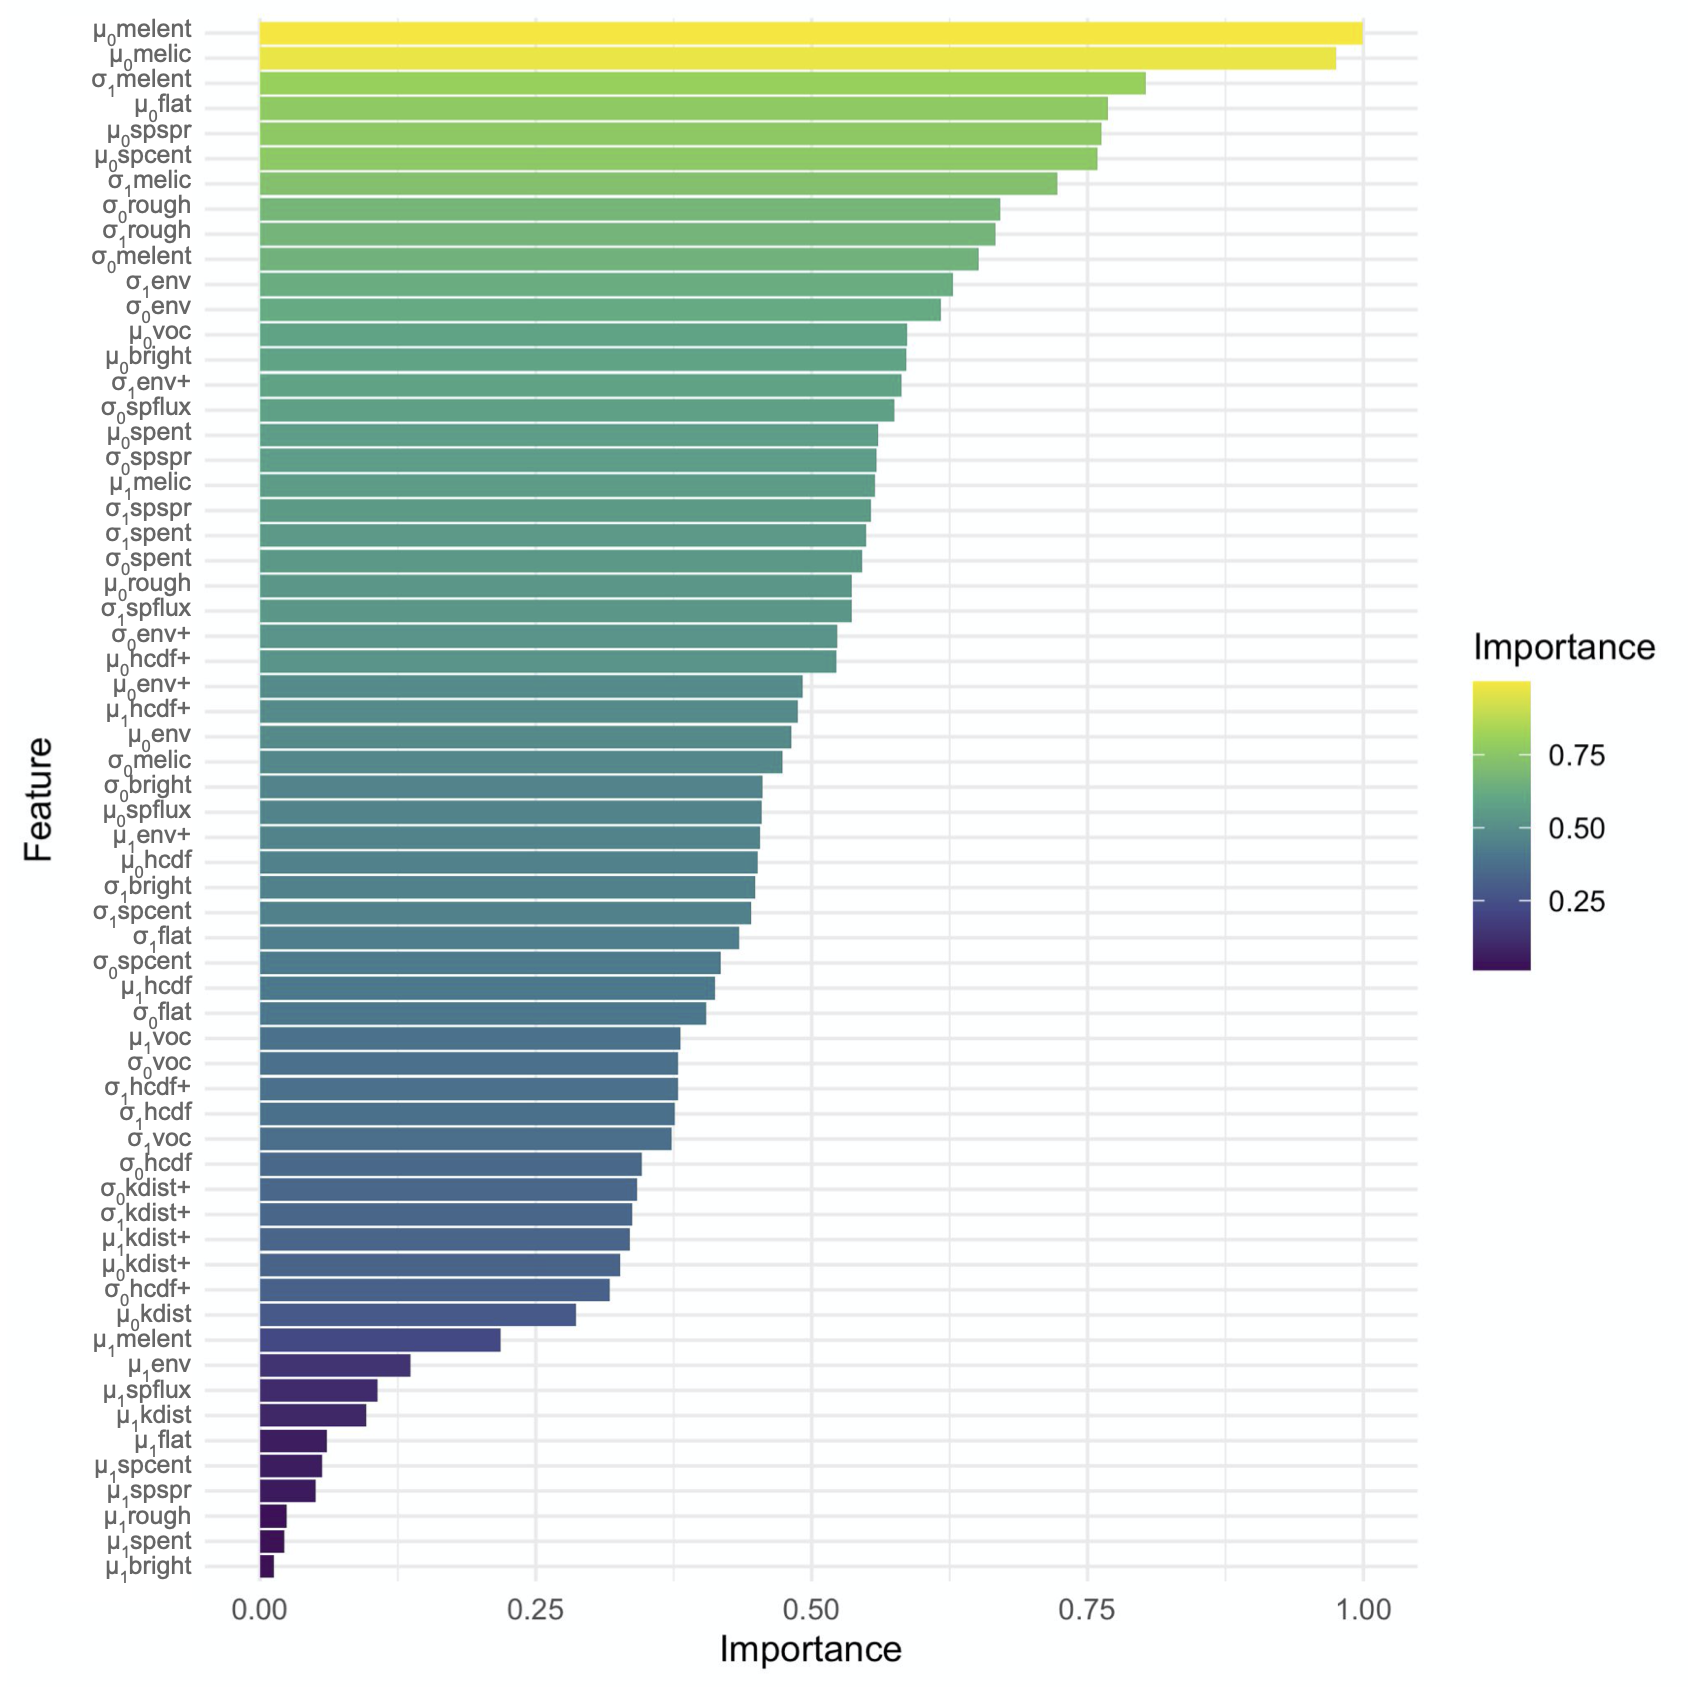
\includegraphics[width=\textwidth]{exp-7.png}
\centering
\caption{Relative feature importance for the SVM trained using all available features. Importance uses an arbitrary scale from 0 to 1, with feature importance rescaled linearly such that the feature contributing the most on each cross-validation fold received a score of 1, as mean melodic entropy did in this case, and the feature contributing the least received a score of 0, which no feature did for all five folds.}
\label{fig:exp-7}
\end{figure}

\section{Discussion}

The permutation tests replicated many of the findings from prior research. Three main types of patterns are identifiable in \autoref{fig:exp-5}: features which were consistently higher than controls around the onset of MECs, features which showed a sharp increase around the onset of MECs, and features which showed no significant differences from controls. First, looking at the original features (as assessed with $\mu_0$), MECs were characterised by elevated brightness, flatness, spectral centroid, spectral entropy, melodic entropy, and presence of vocals, as well as sharp increases in envelope, melodic information content, roughness, spectral flux, spectral spread, and melodic entropy, as well as in envelope and key distance when computed with a larger sliding window. While there were also several frames showing significant differences for the harmonic change detection function (HCDF, and its associated feature computed with a larger sliding window), the overall differences were less convincing than with other features. Interestingly, melodic information content increased around the onset of MECs and decreased afterwards, suggesting the possibility that MECs were associated with a single unexpected event, immediately followed by a return to more expected events. In their study, \textcite{cheung2019} identified that information content and entropy interacted in eliciting pleasure, with chords evoking high degrees of pleasure in contexts with low uncertainty and high surprise, and vice versa. While their experimental paradigm allowed for much more temporal precision than the one presented in this chapter, the very brief decrease in melodic entropy seen in \autoref{fig:exp-5} around the onset of MECs could support the presence of such an interaction.

The variance in these features (as assessed with $\sigma_0$) largely followed similar patterns, with the exception of the presence of vocals, which only contained a single frame with a significant difference between MECs and controls, located at the exact onsets of MECs. We would note that the presence of vocals was the only binary feature in this analysis, and was relatively slow-moving compared to the other features, due to how it was pre-processed. Regardless, this could be interpreted as vocals being more likely around the onsets of MECs (as seen with $\mu_0$), and MECs being slightly but not overly affected by increased variance in the presence of vocals around their onsets. Significant effects were much more sparse when looking at the rate of change of each feature (as assessed with $\mu_1$), with a convincing peak only occurring for the version of envelope computed with a larger sliding window, providing further evidence that sudden, large changes in loudness are associated with MECs. Variance in these rates of change (as assessed with $\sigma_1$) almost exactly followed the variance in the original features (as assessed with $\sigma_0$), which follows the intuition that when variance in a feature is significantly above average, this is also reflected in the variance of its rate of change.

It is worth pointing out that the patterns seen in each feature were of reasonable magnitude, with most differences ranging from 0.1 to 0.3 in Z-scores. It is also worth noting that these were all hypothesised based on previous research rather than exploratory findings. In addition, we applied extremely strict Bonferroni correction, reducing the alpha threshold for statistical significance to slightly higher than 0.001, and therefore providing a high degree of confidence in the identified effects. Tying these results back to findings from prior research (as listed in detail in the introduction and in Chapter \ref{ch:2}), the permutation test analysis provided a large-scale replication of effects showing MECs as being associated with all the acoustic and musical elicitors that were approximated with extracted features, including increases in loudness \parencite[e.g.,][]{sloboda1991}, crescendi \parencite[e.g.,][]{panksepp1995}, increased roughness \parencite[e.g.,][]{grewe2007}, brightness \parencite[e.g.,][]{bannister2018}, event density \parencite[e.g.,][]{nagel2008}, and spectral centroid and flux \parencite[e.g.,][]{bannister2018}, expansion of the frequency range \parencite[e.g.,][]{guhn2007}, and changes in texture, harmony and tonality \parencite[e.g.,][]{sloboda1991}. Finally, we provided novel quantitative evidence for the existence of effects of vocals and of melodic expectation on the occurrence of MECs, which suggests that MECs are more likely in the presence of vocals, and around the onsets of unpredictable notes in uncertain melodic contexts.

Several models were trained to perform automatic MEC onset detection. This resulted in three sets of findings which warrant further discussion. First, we expected HMMs to perform better than SVMs but the opposite was true. As discussed earlier, HMMs are particularly well suited to auditory event detection tasks. However, in prior research, such events were most often well-defined, with precise, objective onsets. Detecting MECs comes with an additional layer of abstraction, with MECs not being detectable directly from the signal, but rather, being psychophysiological reactions to some properties of the signal. In addition, onsets of MECs were gathered from subjective survey answers and therefore did not represent an exhaustive and precise source of ground truth. It is encouraging, however, that prediction performance was relatively comparable between HMMs and SVMs given these limitations, showing that models such as HMMs can be used to detect the onsets of MECs. It could be that HMM performance could be improved by using longer frame sizes and window sizes, for instance, or by better defining an interpretation of the hidden states for each feature. It remains our intuition that sequential models are best suited to the detection of MECs, but successfully applying such methods might rely on obtaining more exhaustive, better-quality data.

Second, while recall was high, precision was very low for all models. Precision, here, refers to the proportion of predicted MECs which were actually MECs, while recall refers to the proportion of MECs in the ground truth which were predicted as MECs. In other words, the models we trained identified a large proportion of the MECs in the ground truth (high recall) but also predicted far too many MECs where none were recorded in the ground truth (low precision). It is worth mentioning, however, that due to the very high class imbalance in the data, baseline precision was extremely low ($P_B$ = 0.011), but all the models still performed better than chance as shown by all AUC values exceeding 0.5. It is because of this low precision that we opted to report results based on the highest F\textsubscript{$\beta$} value returned by each model, since not doing so disproportionately penalised recall by optimising for very small increases in precision. Optimising for recall also made sense, conceptually, due to the nature of the ground truth data. Indeed, since the ground truth data was acquired experimentally, it is highly likely that, with many more participants in the survey, additional onsets of MECs would have been reported for some of the tracks used for model training, which would have occurred during passages categorised as controls in the present analysis. This made the ground truth incomplete, which motivated attempting to predict all the MECs reported in the data by maximising recall, rather than only the MECs present in the data by maximising precision, with the added advantage that an F\textsubscript{$\beta$}-optimised model should provide more useful information about which features best characterised the onsets of MECs when looking at feature importance. While these results are not reported in the present chapter for brevity and clarity, it is also worth mentioning that reporting metrics based on the highest F\textsubscript{$\beta$} value as opposed to the highest F-measure came at almost no cost to precision.

Finally, we found that the models which included IDyOM features in the training set outperformed the models which didn't. While these performance improvements were small, it is worth keeping in mind that, as opposed to the other features which benefited from robust data extraction methods, melodic entropy and information content were both computed based on automatically extracted melodic pitch frequencies---a notoriously difficult and imprecise process subject to much ongoing research---which were then converted to sequences of notes based on a simple heuristic. Despite these limitations, these findings correspond to quantifiable effects of expectation on the occurrence of MECs, which are further reinforced by the findings on feature importance discussed below.

Melodic entropy and information content were indeed the best predictors of MEC onsets by far, followed by the variance in their rates of change as well as the mean of some spectral features (flatness, spread, and centroid). While feature importance is not that informative on its own, it provides interesting insights when combined with the results from the permutation tests, by allowing comparisons between the magnitude of the difference between MECs and controls in each feature, and the degree to which these differences were predictive of MECs. For instance, the lack of detected effects of first-order differences on MECs is also apparent in the fact that most of these features were not strong predictors of MECs. However, these comparisons can be more ambiguous. Many features, such as sharp increases in loudness, benefit from extensive prior empirical support, and strongly displayed the expected behaviour in the permutation tests, but they were not highly ranked in terms of predictive performance. Conversely, the magnitude of the effects detected in the permutation tests for melodic entropy and information content was much lower than for other features, and yet, these expectation-related features were the best predictors of MECs. This suggests that, while previous findings about correlations between various features and MECs were replicated, these features were not always strong predictors of MECs. Taking loudness as an example, it could be that MECs are indeed characterised by sharp increases in loudness, but sharp increases of loudness occur at other moments as well, which makes them inaccurate predictors of MECs. In other words, loudness might be a necessary but non-specific elicitor of MECs. Conversely, small differences in expectation between MECs and controls could be due to small effect sizes, or to increases in entropy and information content only being present in a subset of MEC onsets, but appear to be highly specific to MECs, therefore driving their predictive performance.

Interestingly, \textcite{bannister2020b} found that manipulating loudness and brightness around known onsets of MECs resulted in changes in how many people experienced MECs. Given the results of the feature importance analysis discussed above, a possible interpretation for these causal findings could be that a certain combination of factors is necessary for the occurrence of MECs, as seen by the finding by Bannister that some people reported MECs regardless of loudness and brightness manipulations, but that these manipulations acted upon a loudness and brightness threshold at which different people experience MECs. In other words, it could be that specific levels of loudness and brightness were required for the experience of MECs in some participants, but were not necessarily predictive of such experiences on their own.

It is also worth mentioning a recent article by \textcite{mori2022}, which was published after the present experiment concluded, and featured a very similar methodology to ours. In the study described by the author, 54 participants who often experience MECs were asked to listen to a few self-selected pop rock songs which induce MECs or tears while indicating occurrences of MECs or tears with buttons presses. Acoustic features were extracted using MIRtoolbox, and included most of the acoustic features used in the present analysis, as well as a range of rhythm-related features and mel-frequency cepstral coefficients. Excerpts centred around the onsets of MECs, tears, and a comparable number of randomly selected control excerpts were labelled to train a multi-class ridge regression classifier. Instead of using AUC, predictive performance was assessed with permutation tests, conducted by randomly resampling the predicted labels for each frame to generate a null distribution of predictive accuracies. Feature importance was assessed with bootstrapping---a preferable approach to the one we used, partly because it allows using each feature directly without the need for dimensionality reduction, but which was not practical for our purposes due to our prohibitively computationally expensive model training process.

\textcite{mori2022} obtained a classification accuracy of 43\% around the onsets of MECs, which was significantly better than chance, as revealed by permutation tests. For our best performing model, AUC was 0.597 and balanced accuracy was 58\%, though it is worth pointing out that these numbers are not directly comparable, since \textcite{mori2022} conducted multi-class classification on a balanced dataset, and assessed prediction accuracy with different metrics. In addition, the author identified that these predictions were significantly driven by minor mode immediately preceding MECs (highlighting a possible relationship with expressed valence as seen in Chapter \ref{ch:4}), higher event density and rhythmic entropy at the onset of MECs, and higher spectral flux and rhythmic entropy after the onset of MECs (replicating some of our results as well as some hypothesised effects of rhythmic properties detailed in Chapter \ref{ch:2}). Various mel-frequency cepstral coefficients also significantly predicted MECs, but these provide less room for interpretation. The author conducted an additional study to investigate the effect of lyrical content, as extracted using natural language processing, but found no effect of lyrics on MECs. Overall, \textcite{mori2022} mainly attributed the occurrence of MECs to violations of rhythmic expectation, which is certainly complementary to the present findings about the effects of melodic expectation on MECs.

Our study suffered from a few limitations, the main one being that a model with an AUC below 0.60 is generally considered to be a very poor classifier. However, it is worth placing model performance within the context of the task at hand. As discussed throughout the present chapter, we expected automatic detection of MEC onsets to be far from trivial, due to the inherent impossibility in collecting exhaustive ground truth data, and to MECs being a subjective, psychophysiological response known to be caused by a wide range of elicitors, some of which would be exceedingly difficult to quantify for modelling purposes. Throughout the modelling process, we had to make a lot of necessary decision with little existing basis for an informed choice between the available options. Given this, we aimed to reach a balance between time constraints and informed guesses as to which processing steps would lead to the best chances of success. These decisions were all documented throughout the present chapter in order to provide transparency and enable reproducibility. One decision, notably, was to automatically extract melodic pitch frequency in order to compute expectation-related features. It is highly likely that a replication of the current study using transcribed melodies would lead to a more precise understanding of the effects of expectation on MECs.

More importantly, we wanted our models to be interpretable, which meant that we needed to use both interpretable features, and interpretable models, at the necessary cost of predictive performance. It is highly likely that more powerful approaches, such as neural networks or ensemble methods, using features such as mel-frequency cepstral coefficients as model inputs, would result in better predictive performance. These approaches might gain from some methodological insights gathered in the present study, such as the use of features computed over large sliding windows and segmented using a 500 ms frame size, or the use of segment-based metrics for evaluation. Exploring the benefits of using larger frame sizes might also lead to improved performance. However, we suspect that there is a relatively low ceiling to predictive performance, which, if close to an AUC of 0.60 as seen in the present study, would suggest a more important role of emotional elicitors than previously anticipated. Considering the extent of previous findings about the relationships between MECs and various extra-musical factors such as personal meaning or the state of being moved, it is possible that only a small proportion of MECs are caused by acoustic and musical elicitors via the psychological mechanisms of brain stem reflex and musical expectation (see Chapter \ref{ch:2}). In other words, instead of acoustic, musical, and emotional elicitors equally contributing to the elicitation of MECs through brain stem reflex, musical expectation, and emotional contagion, the low predictive performance of the model could suggest that, in many cases, emotional elicitors are more predictive of the occurrence of MECs. Regardless of which modelling approach is used, future research should seek to empirically validate the models by generating predictions of MECs on a new set of stimuli, and comparing these predictions to reports of MECs collected from new participants.

Another limitation comes from the reliance of the present study on audio feature extraction, notably in terms of perceptual validity. A simplified way to discuss this limitation is by understanding the purposes such features are put to in different disciplines. In music information retrieval, audio features are generally needed to solve computational tasks (such as genre or emotion classification, music similarity quantification, artist identification, etc.) in order to optimise model performance when compared to a relatively objective ground truth. In music psychology, audio features are generally required to understand underlying psychological processes in order to build cognitive models which are evaluated by comparing them to observed behaviour. These distinctions are explored in detail by \textcite{aucouturier2012,aucouturier2013}, and result in different priorities for feature evaluation. In music information retrieval, features are evaluated following a pragmatic process based on whether or not they improve task performance and are computationally simple, whereas in music psychology, feature evaluation is rare, and focuses on whether or not features are interpretable. Some efforts have been made to identify features which approximate the human perception of related psychological constructs, but these are limited by the fact that they are not easily computable for use in other studies \parencite[e.g.,][]{aljanaki2018,friberg2014}. It is therefore very common in psychology experiments to extract features using existing music information retrieval toolboxes---as a very crude example, MIRtoolbox \parencite{lartillot2008} has been cited in more than 600 articles including the word \emph{psychology}---seeing as the need for computational features often exceeds the need for the perceptual validity provided by subjective ratings, as was the case in the present study. Perceptual validation of audio features would greatly improve the interpretability of the present research, and of research in music psychology in general, but such work would represent a considerable undertaking. In the meantime, and despite their advantages, using audio features to model psychophysiological responses such as MECs should come with the understanding that these features should not be equated with the human perception of related constructs.

In summary, we conducted a set of computational analyses, resulting in a large-scale replication of previous findings about acoustic and musical elicitors of MECs, and in the construction of a model which can identify onsets of MECs better than chance. The hypothesised role of expectation in the experience of MECs was confirmed in a series of novel empirical findings, showing that melodic entropy and information content were significantly different between MECs and controls, led to increased predictive performance when included during model training, and were the best predictors of MEC onsets. Future research should seek to explore the many remaining gaps in knowledge about the relationship between expectation and MECs. Notably, questions remain about the exact interaction between uncertainty and surprise, the role of harmonic expectation, and the differences between schematic and veridical expectation.
